
\begin{savequote}[75mm]
	The only way to learn mathematics is to do mathematics.
	\qauthor{--- Paul Halmos ---}
\end{savequote}

\chapter{Sets and numbers}
\graphicspath{{figures/Sets/}}
\label{SetsChapter}
\ifcourse
To make sure that everyone has an understanding of the basic concepts that are at the basis of subsequent chapters, we begin this part with a brief summary of set theory and some of the associated vocabulary and notations we use throughout the text. 
\fi

\ifvc
We begin with a brief summary of set theory and some of the associated vocabulary and notations we use throughout the text. 
\fi

\section{Sets}
\label{sets}
\subsection{Logic operators}
\label{sec:logic operators}
Throughout this course, and especially when defining new mathematical objects, we will often make use of notation that contains one or more logic operators. An overview of them is given in Table~\ref{tab:logicsymbols}. Note the difference between $X \Rightarrow Y$ and $X \Leftrightarrow Y$. $X \Rightarrow Y$ states that if $X$ is true, $Y$ is also true, but if $Y$ is true, $X$ is not necessarily true. $X \Leftrightarrow Y$, on the other hand, states that $X$ and $Y$ are both true or both not true and thus equivalent. For instance, we may write
$$
\text{Garfield is a cat } \wedge\text{ all cats are mammals }  \Rightarrow \text{ Garfield is a mammal}\,,
$$
though 
$$
\text{Garfield is a mammal }  \not\Rightarrow \text{ Garfield is a cat}\,!
$$


\begin{table}[]
	\centering
	\renewcommand{\arraystretch}{2}%
	\begin{tabular}{c||c}
		Notation               & Reads as \\\hline
		$X \Rightarrow Y$     & $X$ implies $Y$;  if $X$ then $Y$\\\hline
		$X \Leftrightarrow Y$  & $X$ if and only if $Y$\\\hline
		$X \wedge Y$           & $X$ and $Y$ \\\hline
		$X \vee Y$             & $X$ or $Y$ \\\hline
		$\forall x$   & for all (elements) $x$ \\\hline
		$\exists x$   & there exists an (element) $x$ \\\hline
		$\exists !\  x$   & there exists just one (element) $x$ \\\hline
		$.|.$   & . so that . \\\hline
		$:.$   & it holds that . \\
	\end{tabular}
	\caption{Overview of important logic operators. $X $ and $Y$ denote logic statements, which are either true or false.}
	\label{tab:logicsymbols}
\end{table}


\pagebreak
\subsection{Definition and representation of sets}
We start with a definition of a set. 
\begin{definition}[Set]
A \textbf{set}\index{set}\index[aut]{verzameling} (\textit{verzameling}) is a well-defined collection of objects which are called the elements of the set.  
\end{definition}
In this definition, `well-defined' means that it is possible to determine if something belongs to the collection or not, without prejudice. For example, the collection of letters that make up the word `smolko' is well defined and is a set, but  the collection of the worst math teachers in the world is not well defined, and so is not a set.  In general, there are three ways to describe sets. 

\begin{enumerate}
	\item The \textbf{verbal method}: use a sentence to define a set.
	\item The \textbf{roster method}:  begin with a left brace `$\{$', list each element of the set only once and then end with a right brace `$\}$'.
	\item The \textbf{set-builder method}: a combination of the verbal and roster methods.
\end{enumerate}
\index{verbal method}
\index{roster method}
\index{set-builder notation}

For example, let $S$ be the set described verbally as the set of letters that make up the word `smolko'.  A  roster description of $S$ would be  $S=\left\{ s, m, o, l, k \right\}$. Note that sets do not allow for repeated elements while they are also  orderless, so $\left\{ k,  l,  m, o, s \right\}$ is also a roster description of $S$. A set-builder description of $S$ is: 
\[ S=\{ x \, | \, \mbox{$x$ is a letter in the word `smolko'}\}. \]

In this notation we call $x$ a \textbf{dummy variable} and `$x$ is a letter in the word `smolko'' the \textbf{predicate}. The way to read this is: `The set of elements $x$ such that $x$ is a letter in the word `smolko.'
%Actually, proceeding in this way it is implicitly understood that the predicate should be interpreted with respect to the letters available in the European alphabet.  This alphabet may hence be understood as the universal set in which the predicate must be interpreted. In the case of ambiguity this can be made more explicit in the set-builder description as
%\[ S=\{ x \in \mbox{European alphabet}\, | \, \mbox{$x$ is a letter in the word `smolko'}\}. \]
Clearly $m$ is in $S$ and $q$ is not in $S$, i.e.\   $m \in S$ and $q \notin S$.  Moreover, the empty set is written as $A=\left\{\right\}$ or $A=\emptyset$, and a set containing a single element is reffered to as a \textbf{singleton} (\textit{singleton}).
\index{dummy variable}\index[aut]{dummy variabele}
\index{predicate}\index[aut]{predicaat}
\index{singleton}\index[aut]{singleton} 

Graphically, sets are typically represented by means of so-called \textbf{Venn diagrams} (\textit{Venn-diagram}), enclosed areas in the plane. For instance, Figure~\ref{fig_sets_1} shows the Venn diagram of the set $S=\left\{ s, m, o, l, k \right\}$. \index{Venn diagram}\index[aut]{Venn-diagram}


\begin{figure}[h!]
	\begin{center}
		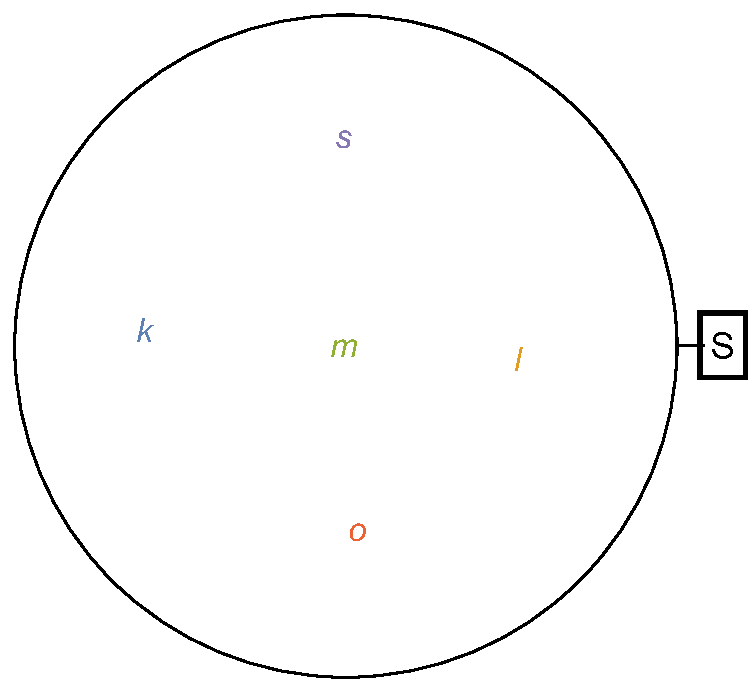
\includegraphics[width=0.3\textwidth]{fig_sets_1}
		\caption{Venn diagram of the set $S=\left\{ s, m, o, l, k \right\}$.}
		\label{fig_sets_1}
	\end{center}
\end{figure}

\ifcourse
\ifanalysis

	The fact that a set sensu stricto does not bear an ordering constitutes an inconvenience in  applications where one may often easily envisage an order relation to order the elements in a particular set.  In this way, one arrives at a so-called ordered set, which is formally defined below. 
	\\
	
	\begin{definition}[Ordered set]
		An \textbf{ordered set} (\textit{geordende verzameling}) is a set $S$, together with
		a relation $<$ such that
		\begin{enumerate}
			\item For any $x, y \in S$, exactly one of
			$x < y$, $x=y$, or $y < x$ holds.
			\item If $x < y$ and $y < z$, then $x < z$.
		\end{enumerate}
		We write $x \leq y$ if $x < y$ or $x=y$. Besides, we may define
		$>$ and $\geq$ in a similar way.
		\index{set ! ordered}
		\index[aut]{verzameling ! geordend}
	\end{definition}
	For example, the set of countries can be ordered by landmass, so India $>$ Lichtenstein. Likewise, the dictionary is the ordered set of words where the order is the so-called lexicographic ordering.  In the remainder of this course, we will, however, mostly be interested in ordered
	sets of numbers.

\fi
\fi

\subsection{Set operations}
\label{setoperations}
Having defined sets, we can now devise some operations that can be performed with them. Let us consider two sets $A$ and $B$. First, we define that  $A$ and $B$ are equal if and only if they have the same elements, that is
$$
(A=B) \quad\Leftrightarrow\quad \left(\forall x\mid  (x\in A) \Leftrightarrow (x\in B)\right)\,.
$$


The equality of two sets can be expressed alternatively upon introducing the concept of \textbf{subsets} (\textit{deelverzameling}). We say that $A$ is a subset of the set $B$,  if all elements of $A$ are in $B$; that is if and only if $\forall x: x\in A\Rightarrow x\in B$. We write this as $A\subseteq B$. It immediately follows that two sets $A$ and $B$ are equal if and only if $A\subseteq B$ and $B\subseteq A$. A \textbf{proper subset} (\textit{strikte deelverzameling}) $A$ of a set $B$, denoted $A\subset B$, is a subset that is strictly contained in $B$ and so necessarily excludes at least one element of $B$. 

\ifcourse

\begin{remark}[Equality]
	Robert Recorde, a Welsh mathematician, introduced the equal sign in 1557. He motivated his choice, by stating: 
	\textit{And to avoid the tedious repetition of these words: is equal to: I will set as I do often in work use, a pair of parallels, or Gemowe lines of one length, thus: $=$, because no 2 things, can be more equal.}	
\end{remark}
\fi

\ifcourse
\ifanalysis

	Mathematically, we may write
	$$
	\left(A\subset B\right) \quad\Leftrightarrow\quad  \big(\left(A\subseteq B\right) \, \land \, \left(A\neq B\right)\big)\,.
	$$

\fi
\fi

For instance, the regular polygons make up a proper subset of the set of polygons. %(Figure~\ref{fig_sets_3}).
\index{subset}\index[aut]{deelverzameling}
\index{subset ! proper}\index[aut]{deelverzameling ! strikt}

% \begin{figure}[h!]
% 	\begin{center}
% 		\includegraphics[width=0.4\textwidth]{fig_sets_3_cropped}
% 		\caption{The regular polygons make up a proper subset of the set of polygons.}
% 		\label{fig_sets_3}
% 	\end{center}
% \end{figure}

Finally, we can define a \textbf{universal set} (\textit{universum}), often denoted by $U$, which contains all objects, including itself.
Actually, in the set-builder description of the exemplary set $S=\left\{ s, m, o, l, k \right\}$, it is implicitly understood that the predicate should be interpreted with respect to the letters available in the European alphabet.  This alphabet may hence be understood as the universal set in which the predicate must be interpreted. In the case of ambiguity this can made more explicit in the set-builder description as
\index{universal set}\index[aut]{universum}

\[ S=\{ x \in \mbox{European alphabet}\, | \, \mbox{$x$ is a letter in the word `smolko'}\}. \]

% BIOIR: MEER DEFINITIE GEBASEERD

Let us now envisage the following operations on the sets $A$ and $B$, subsets of the universal set $U$, which are illustrated in Figure~\ref{fig_sets_2}.


\begin{figure}[t]
	\centering
	%\raisebox{0.5cm}{
	\centerline{
		\subfigure[Intersection \label{fig_sets_2a}]{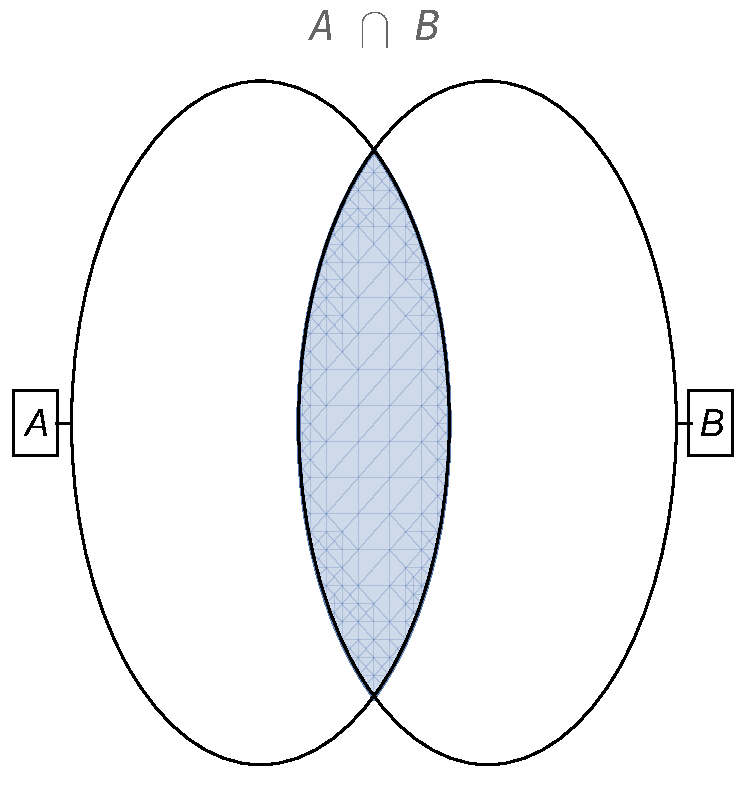
\includegraphics[width=0.3\textwidth]{fig_sets_2a}}
		\hspace{1cm}
		\subfigure[Union \label{fig_sets_2b}]{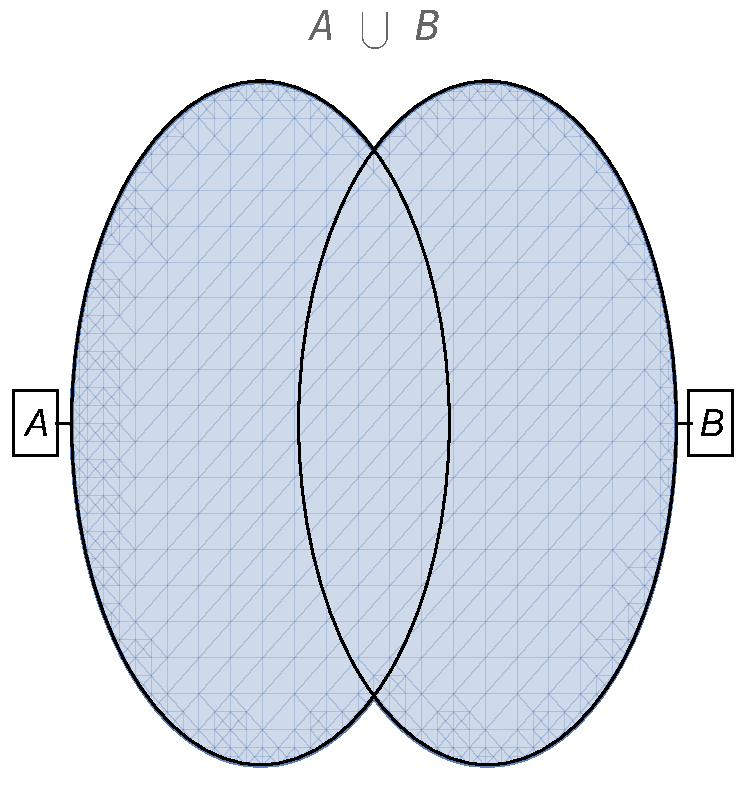
\includegraphics[width=0.3\textwidth]{fig_sets_2b}}
		\hspace{1cm}
		\subfigure[Complement \label{fig_sets_2c}]{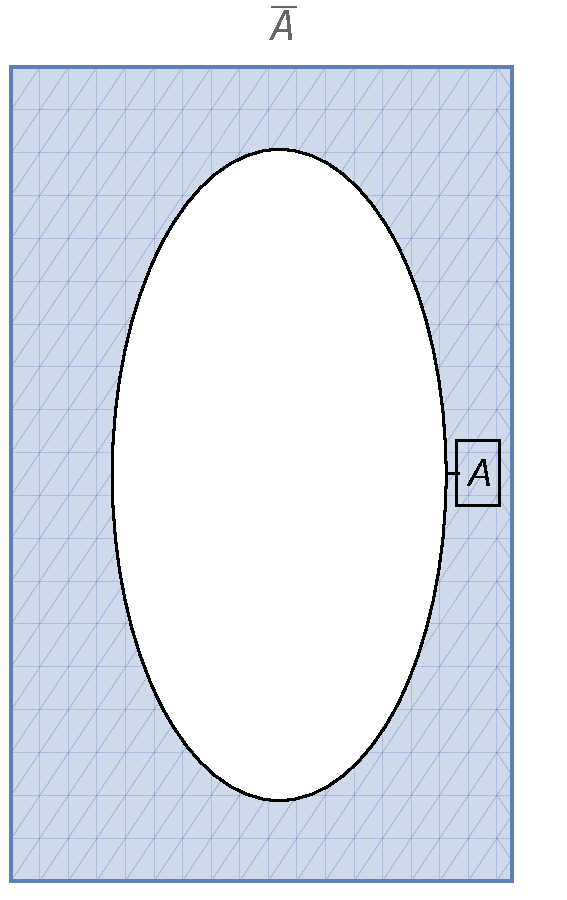
\includegraphics[width=0.2\textwidth]{fig_sets_2c}}
	}
	\centerline{
		\subfigure[Difference \label{fig_sets_2d}]{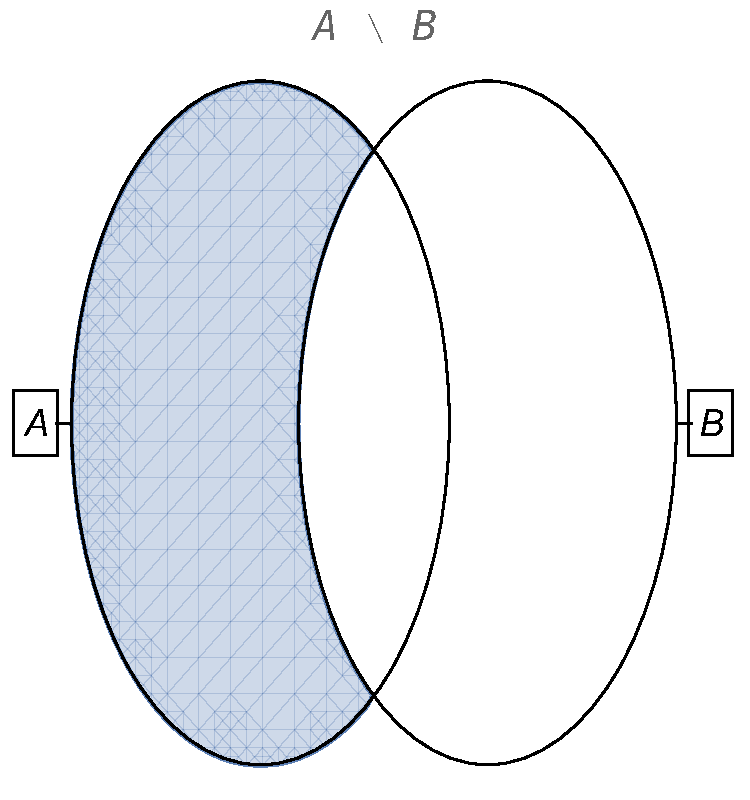
\includegraphics[width=0.3\textwidth]{fig_sets_2d}}
		\hspace{1cm}
		\subfigure[Symmetric difference \label{fig_sets_2e}]{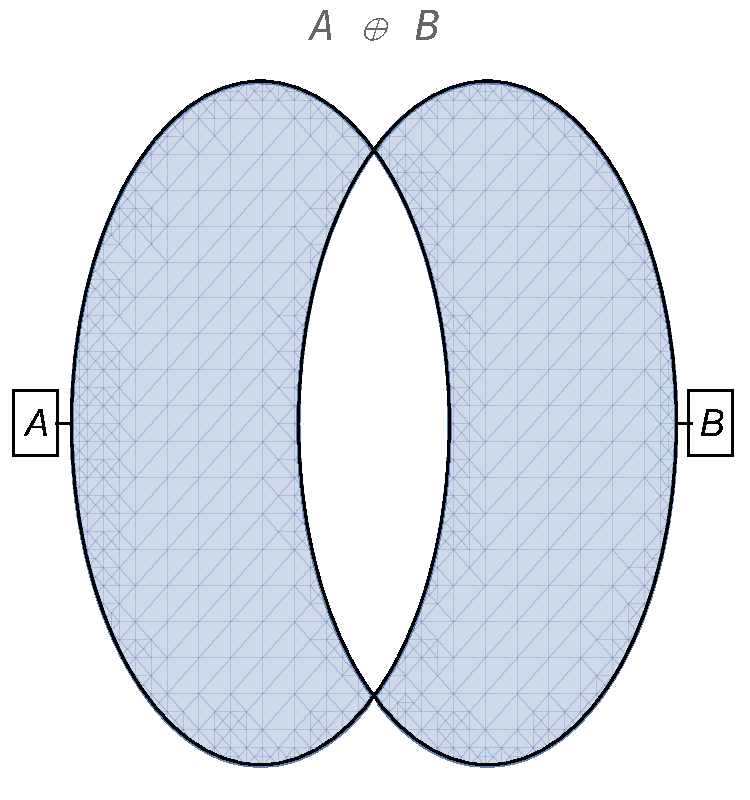
\includegraphics[width=0.3\textwidth]{fig_sets_2e}}
	}
	\caption{Set operations involving two sets $A$ and $B$.\label{fig_sets_2}} 
	
\end{figure}

\begin{itemize}
	\item \textbf{Intersection} (\textit{doorsnede}): \index{intersection}\index[aut]{doorsnede}
	$$
	A\cap B=\left\{x\mid \left(x\in A\right)\wedge\left(x\in B\right)\right\}.
	$$
	This yields the common elements of $A$ and $B$. Two sets are called \textbf{disjoint} (\textit{disjunct}) if $A\cap B=\emptyset$. This operation generalises directly to $n$ sets. \index{disjoint}\index[aut]{disjunct}
	\item \textbf{Union} (\textit{unie}): \index{union}\index[aut]{unie} 
	$$
	A\cup B=\left\{x\mid \left(x\in A\right)\vee\left(x\in B\right)\right\}.
	$$
	This yields the set of elements that belong to either of the two sets. This operation generalises directly to $n$ sets. 
	\item \textbf{Complement} (\textit{complement}): \index{complement}\index[aut]{complement}  
	$$
	\overline{A}=\left\{x\in U\mid x\notin A \right\}.
	$$
	This yields the set of elements in the universal set $U$ that do not belong to a set $A$.
	\item \textbf{Difference} (\textit{verschil}): \index{difference}\index[aut]{verschil}
	\ifvc
	$$
	A\setminus B=\left\{x\mid \left(x\in A\right)\wedge\left(x\notin B\right)\right\}=A\cap\overline{B}.
	$$
	This yields the set of elements that belong to set $A$ but not to set $B$. 
	\fi
	\ifcalculus
	$$
	A\setminus B=\left\{x\mid \left(x\in A\right)\wedge\left(x\notin B\right)\right\}=A\cap\overline{B}.
	$$
	This yields the set of elements that belong to set $A$ but not to set $B$. 
	\fi
	
	\ifanalysis
	
		$$
		A\setminus B=\left\{x\mid \left(x\in A\right)\wedge\left(x\notin B\right)\right\}.
		$$
		This yields the set of elements that belong to set $A$ but not to set $B$. There is also a relationship between the set difference and set complement, which can be understood from the following:
		\begin{eqnarray*}
			A \setminus B&=& \left\{x\mid \left(x \in A\right) \land \left(x \notin B\right)\right\}\\
			&=& \left\{x\mid \left(x \in A \wedge x \in U\right)  \land \left(x \notin B\right)\right\}\\
			&=& \left\{x\mid \left(x \in A \right)\wedge \left( x \in U  \land x \notin B \right)\right\}\\
			&=& \left\{x\mid \left(x \in A\right) \wedge  \left(x \in  \overline{B}\right) \right\}\\
			&=& A\cap\overline{B}\,.
		\end{eqnarray*}
	
	\fi
	

	
	\item \textbf{Symmetric difference} (\textit{symmetrisch verschil}): \index{symmetric difference}\index[aut]{symmetrisch verschil}
	$$
	A\oplus B=\left\{x\mid \left(x\in A\cup B\right)\wedge \left(x\notin A\cap B\right)\right\}.
	$$
	%\todo[inline,backgroundcolor=green!25]{$A\oplus B=\left\{x\mid \left(x\in A\cup B\right)\wedge \left(x\notin A\cap B\right)\right\}\,.$}
	This yields the set of elements that belong to either one or the other set but not both.
	
	\item \textbf{Cartesian product} (\textit{Cartesisch product}): \index{Cartesian product}\index[aut]{Cartesisch product}
	$$
	A\times B=\left\{\left(a,b\right)\mid \left(a\in A\right)\wedge\left(b\in B\right)\right\}.
	$$
	This yields the set of ordered pairs of $\left(a,b\right)$ of all elements $a$ and $b$, that belong to set $A$ and $B$, respectively. When taking the Cartesian product of $A$ with itself, i.e.\ $A\times A$, this is also denoted as $A^2$.
\end{itemize}




\ifcourse
\begin{remark}[Venn-diagrams]
	Venn diagrams were named after John Venn (1843--1923), who studied and standardised these diagrams.
	A major issue that he tried to tackle, was finding symmetrical diagrams of partially multiple overlapping sets. Venn only got as far as 4 sets and it took until 1975 for mathematicians to extend this to 5 and more. The figure below illustrates this for 5, 7 and 11 sets, respectively. %\textbf{(ref: MathWorld)}.
	%Ref: Weisstein, Eric W. "Venn Diagram." From MathWorld--A Wolfram Web Resource. http://mathworld.wolfram.com/VennDiagram.html
	\begin{center}
		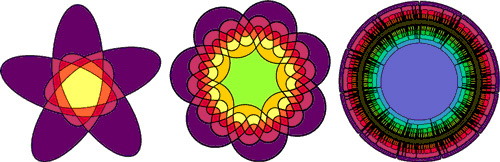
\includegraphics[width=0.5\textwidth]{fig_sets_3.jpg}
		%\caption{Symmetric Venn diagrams of 5, 7 and 11 overlapping seys.}
	\end{center}
	
\end{remark}
\fi


\ifvc
\begin{example}
	Consider the following three sets that contain words from three Germanic languages, namely Dutch, English and German, respectively:
	\begin{eqnarray*}
		D&=&\left\{\mbox{Afrikaans, computer, duif, fiets, internet, \"uberhaupt}\right\},\\
		E&=&\left\{\mbox{Afrikaans, bike, blitzkrieg, computer, fest, internet, pigeon}\right\},\\
		G&=&\left\{\mbox{blitzkrieg, computer, fest, internet, rad, taube, \"uberhaupt}\right\}.
	\end{eqnarray*}
	\begin{enumerate}
		\item Construct the Venn diagram representation of the three sets. 
		\item Determine the set $D_1$ of words that appear in Dutch only.
		\item Determine the set $D_2$ of words that are common to both English and German, but not to Dutch. 
		\item Determine the Cartesian product of $D_1\times D_2$ and $D_1\times D_1$.
	\end{enumerate}
	
	\xhrulefill{gray}{2.5pt}Solution \xhrulefill{gray}{2.5pt}
	
	\begin{enumerate}
		\item Figure~\ref{fig_sets_4} shows the Venn diagram of the three sets. 
		\begin{figure}[H]
			\begin{center}
				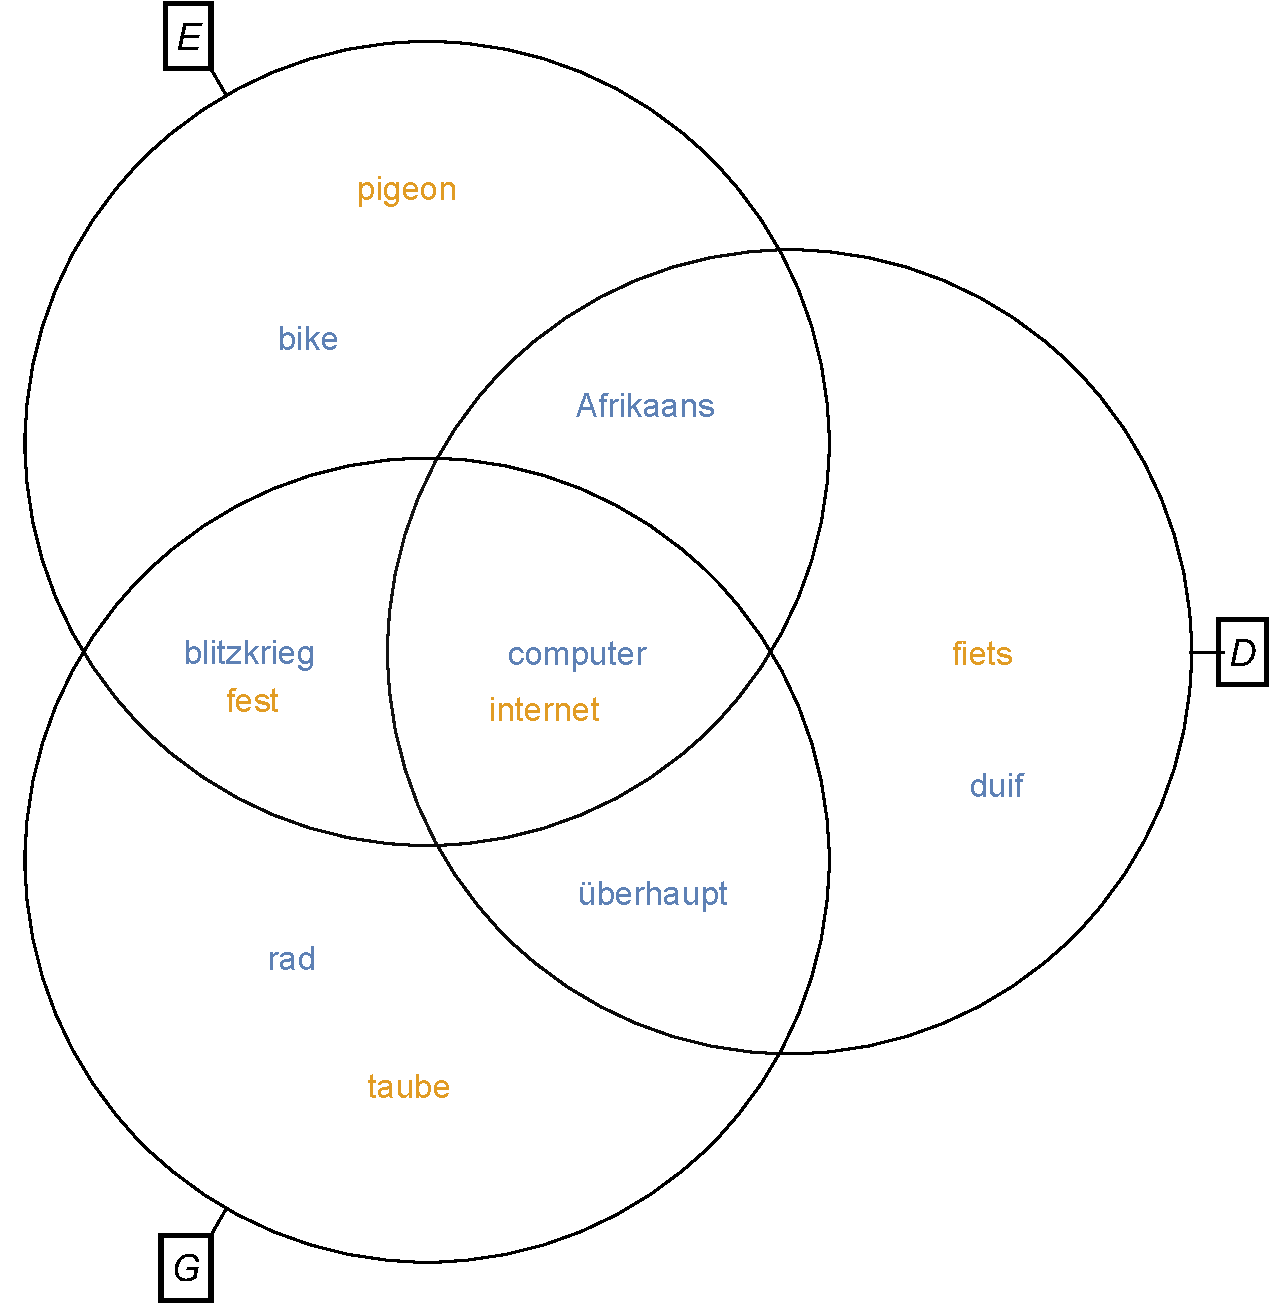
\includegraphics[width=0.4\textwidth]{fig_sets_4}
				\caption{Venn diagram of the sets $D$, $E$ and $G$.}
				\label{fig_sets_4}
			\end{center}
		\end{figure}
		
		\item \label{setexampleD1} The set of words that appear in Dutch only, is nothing but the set of all Dutch words minus the set of words that appear either in German or English. More formally, we can define this set as
		$$
		D_1=D\setminus \left(G\cup E\right)=\left\{\mbox{duif, fiets}\right\}.
		$$
		\item \label{setexampleD2} The set of words that are common to both English and German, but not to Dutch,  can be found by excluding Dutch words from the intersection of $E$ and $G$. Hence, we get
		$$
		D_2=(E\cap G)\setminus D=\left\{\mbox{blitzkrieg, fest}\right\}.
		$$
		
		\item  The Cartesian products follow immediately using $D_1$ and $D_2$ determined in 2 and 3: 
		$$
		D_1 \times D_2 = \left\{\left(\mbox{duif, blitzkrieg}\right), \left(\mbox{duif, fest}\right), \left(\mbox{fiets, blitzkrieg}\right), \left(\mbox{fiets, fest}\right)\right\},
		$$
		
		$$
		D_1^2 = \left\{\left(\mbox{duif, duif}\right), \left(\mbox{duif, fiets}\right), \left(\mbox{fiets, duif}\right), \left(\mbox{fiets, fiets}\right)\right\}.
		$$
	\end{enumerate}
	
\end{example}

\fi


\subsection{Set properties}
Below we list the most important properties of sets, most of which can be understood intuitively or using a Venn diagram representation.
\index{commutativity}\index[aut]{commutativiteit}\index{associativity}\index[aut]{associativiteit}\index{distributivity}\index[aut]{distributiviteit}
\begin{itemize}
	\item \textbf{Commutativity} (\textit{commutativiteit}) of intersection and union:
	$$
	A\cap B=B\cap A \quad\mbox{ and }\quad A\cup B=B\cup A.
	$$
	\item \textbf{Associativity} (\textit{associativiteit})  of intersection and union:
	$$
	A\cap \left(B\cap C\right)=\left(A\cap B\right)\cap C \quad\mbox{ and }\quad A\cup \left(B\cup C\right)=\left(A\cup B\right)\cup C.
	$$
	\item \textbf{Distributivity} (\textit{distributiviteit})  with respect to intersection and union:
	$$
	A\cup \left(B\cap C\right)=\left(A\cup B\right)\cap \left(A\cup C\right) \quad\mbox{ and }\quad A\cap \left(B\cup C\right)=\left(A\cap B\right)\cup \left(A\cap C\right).
	$$
	\item \textbf{Identity laws}:
	$$
	A \cup \emptyset =A \quad\mbox{ and }\quad A \cap U= A.
	$$
	\item \textbf{Complement laws}:
	$$
	A \cup \overline {A} =U \quad\mbox{ and }\quad A \cap \overline {A} = \emptyset. 
	$$
\end{itemize}
For instance, if we are looking for the words that are common to Dutch, English and German, it does not matter that we first determine the words that are common to Dutch and English and then look which of those also are used in German, or start by first determining the words that are common to German and English and finally verify which of those are also used in Dutch. 

For completeness, we also mention the \textbf{De Morgan's laws} (\textit{regels van De Morgan}):\index{De Morgan's laws}\index[aut]{De Morgan ! regels van}
$$
\overline{A\cup B}=\overline{A}\cap\overline{B} \quad\mbox{ and }\quad\overline{A\cap B}=\overline{A}\cup\overline{B}.
$$

\ifcourse
\ifanalysis

	When considering ordered sets, we are often interested in the elements lying at their  boundaries.\\
	
	\begin{definition}[Upper bound, lower bound, supremum, infimum]
		\label{sup_def}
		Let $A \subset S$, where $S$ is an ordered set.
		
		\begin{enumerate}
			\item If there exists a $b \in S$ such that $x \leq b$ for all $x \in A$, then we say $A$ is \textbf{bounded above} (\textit{naar boven begrensd}) and $b$
			is an \textbf{upper bound} (\textit{bovengrens}) of $A$.
			\item If there exists a $a \in S$ such that $x \geq a$ for all $x \in A$,
			then we say $A$ is \textbf{bounded below} (\textit{naar beneden begrensd}) and $a$
			is a \textbf{lower bound} (\textit{ondergrens}) of $A$.
			\item If there exists an upper bound $\beta$ of $A$ such that whenever
			$b$ is any upper bound for $A$ we have $\beta \leq b$, then $\beta$
			is called the \textbf{least upper bound} (\textit{kleinste bovengrens}) or
			the \textbf{supremum}
			of $A$.    We write
			\begin{equation*}
			\sup\, A = \beta .
			\end{equation*}
			This is illustrated in Figure~\ref{fig_sets_5}.
			\item Similarly, if there exists a lower bound $\alpha$ of $A$ such that whenever
			$a$ is any lower bound for $A$ we have $\alpha \geq a$, then $\alpha$
			is called the \textbf{greatest lower bound} (\textit{grootste ondergrens}) or
			the \textbf{infimum}
			of $A$.  We write
			\begin{equation*}
			\inf\, A = \alpha  .
			\end{equation*}
		\end{enumerate}
		When a set $A$ is both bounded above and bounded below, we say simply that
		$A$ is \textbf{bounded} (\textit{begrensd}).
	\end{definition}
	\index[aut]{bovengrens}
	\index[aut]{ondergrens}
	\index[aut]{supremum}
	\index[aut]{infimum}
	\index{upper bound}
	\index{lower bound}
	\index{supremum}
	\index{infimum}

	
	
	
	It should be stressed that the supremum (or infimum) is automatically unique (if it exists).  Indeed, if $\beta$ and
	$\beta'$ are both suprema of $A$, then $\beta \leq \beta'$ and $\beta' \leq \beta$, because both $\beta$ and $\beta'$ are the least upper bounds, so it must hold that $\beta=\beta'$. For instance, let $S := \{ a, b, c, d, e \}$ be ordered as $a < b < c < d < e$, and let $A := \{ a, c \}$.  Then $c$, $d$, and $e$ are upper bounds of $A$, and $c$ is the -- unique -- least upper bound or supremum of $A$. Likewise, the infimum of  $\{2,3,4\}$ is 2. 
	\begin{figure}[h]
		\begin{center}
			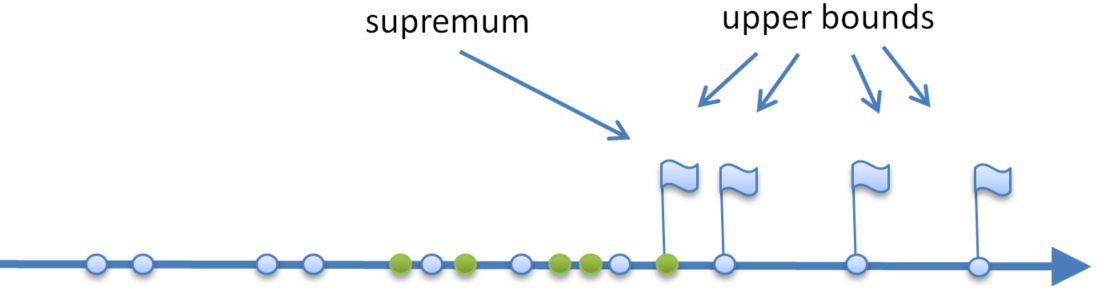
\includegraphics[width=0.6\textwidth]{fig_sets_5}
			\caption{Upper bounds and the supremum of an ordered set $A\subset S$, where the ordering is endowed by the axis and the elements of $A$ are shown as green dots.}
			\label{fig_sets_5}
		\end{center}
	\end{figure}
	
\index{minimum}
\index{maximum}
\index[aut]{minimum}
\index[aut]{maximum}
	Finally, it should be noted that a supremum or infimum for $A$ (even if they exist) need not be in $A$. If $\sup \, A \in A$, then we also denote it by $\max\, A$ and call it the \textbf{maximum} (\textit{maximum}) of $A$, and likewise if $\inf\, A\in A$, then we also denote it by $\min\, A$ and call it the \textbf{minimum} (\textit{minimum}) of $A$. For 
	
	\begin{example}
		Let us consider the set
		$$
		A=\left\{\dfrac{1}{n}\bigg| n=1,2,3,\ldots\right\}\,.
		$$ 
		Then it holds that $\sup\, A = 1$ and since this supremum belongs to
		$A$, we say that $\max\, A =1$. On the other hand, $\inf\, A = 0$ does not belong to $A$, so $A$ has no minimum.
	\end{example}
	
	We conclude this section with an important property that a set may have as it is at the basis of some of the proofs in the upcoming chapters. 
	\begin{definition}[Least-upper-bound property] \label{defn:lub}
		An ordered set $S$ has the \textbf{{least-upper-bound property}} (\textit{supremumeigenschap}) if
		every nonempty subset $A \subset S$ that is bounded above has a least upper bound, that is $\sup\, A$ exists in $S$.
	\end{definition}
	
	The least-upper-bound property is sometimes called the \textbf{completeness property}.
	

\fi
\fi


\section{The set of real numbers}
\label{sec_real}
\subsection{Definition}

Throughout your mathematical upbringing, you have encountered several famous sets of numbers:  
\begin{itemize}
	\item The set of  \textbf{natural numbers} (\textit{natuurlijke getallen}):  $\mathbb N= \{ 0, 1, 2, 3,  \ldots\}$.
	%\item The set of \textbf{whole numbers}: $\mathbb W= \{ 0, 1, 2, 3,  \ldots\}$.
	\item The set of \textbf{integers} (\textit{gehele getallen}): $\mathbb Z=\{ \ldots, -3, -2, -1, 0, 1, 2, 3, \ldots \}$.
	\item The set of \textbf{rational numbers} (\textit{rationale getallen}): $$\mathbb Q=\left\{\dfrac{a}{b} \, \bigg| \, a,b  \in \mathbb Z \, \wedge \, b \neq 0 \right\}\,.$$
\end{itemize}
Essentially, rational numbers are the ratios of integers, provided the denominator is not zero. For instance, 
$$
\dfrac{3}{4}=0.75, \qquad \mbox{and}\qquad \dfrac{1}{3}=0.333333\ldots
$$
are just two exemplary rational numbers.  Looking at those, it is clear that another way to describe the rational numbers is:
\[\mathbb Q=\{x\,|\,\mbox{$x$ possesses a repeating or terminating decimal representation}\}.\]
Indeed, it can be proofed that any decimal number with a repeating or terminating decimal representation can be written as a ratio of integers, so as a rational number. 

\index{natural number}\index[aut]{natuurlijk getal}
\index{integer}\index[aut]{geheel getal}
\index{rational number}\index[aut]{rationaal getal}
\index{number ! natural}\index[aut]{getal ! natuurlijk}
\index{number ! integer}\index[aut]{getal ! geheel}
\index{number ! rational}\index[aut]{getal ! rationaal}

There are of course numbers with a decimal that neither repeats nor terminates, e.g.  
$$
\pi=3.141592654\ldots, \qquad \mbox{and}\qquad 0.123456789101112123\ldots
$$
Such numbers are called \textbf{irrational numbers} (\textit{irrationale getallen}) and they form the set of the irrational numbers, denoted $\mathbb{I}$. Now, we can define a new set, namely the set of so-called \textbf{real numbers} (\textit{re\"ele getallen}) as follows:
\index{real number}\index[aut]{re\"eel getal}
\index{irrational number}\index[aut]{irrationaal getal}
$$
\mathbb{R}=\mathbb{I}\cup\mathbb{Q}\,.
$$
Figure~\ref{fig_sets_6} shows how the sets of natural, rational and real numbers are nested. It clearly holds that the set of natural numbers is a proper subset of the one of the integers, which on its turn is again a proper subset of the set of rational numbers, and so on. Besides, this Venn diagram emphasizes that the sets of rational and irrational numbers are disjoint. 


\begin{figure}
	\begin{center}
		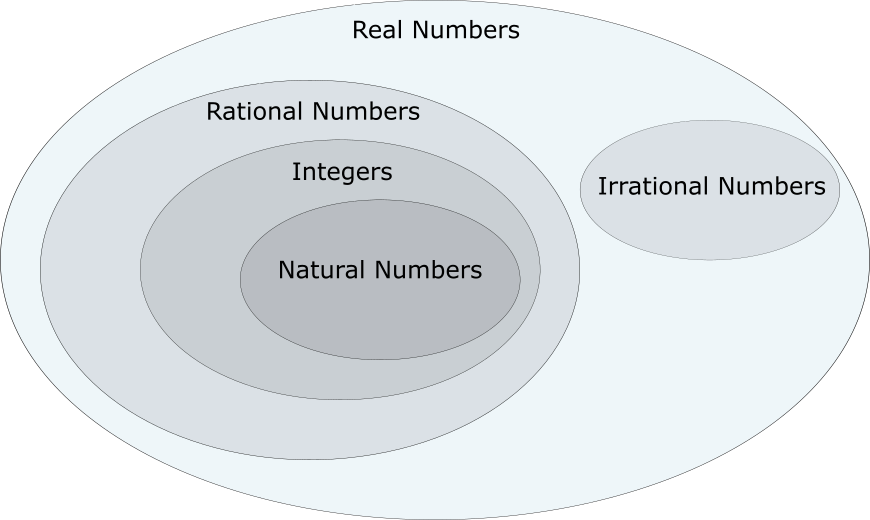
\includegraphics[width=0.4\textwidth]{fig_sets_6}
		\caption{Venn diagram of the sets of natural, integer, rational, irrational and real numbers.}
		\label{fig_sets_6}
	\end{center}
\end{figure}

\index{irational number}\index[aut]{irrationaal getal}
\index{real number}\index[aut]{re\"eel getal}
\index{complex number}\index[aut]{complex getal}
\index{number ! irational}\index[aut]{getal ! irrationaal}
\index{number ! real}\index[aut]{getal ! re\"eel}


The set $\mathbb R$ may be visualized as a line because its elements can be ordered using an order relation. More precisely, the real numbers can be identified with the points on an infinitely long line once its origin, unit of length and orientation have been chosen:
\begin{center}
	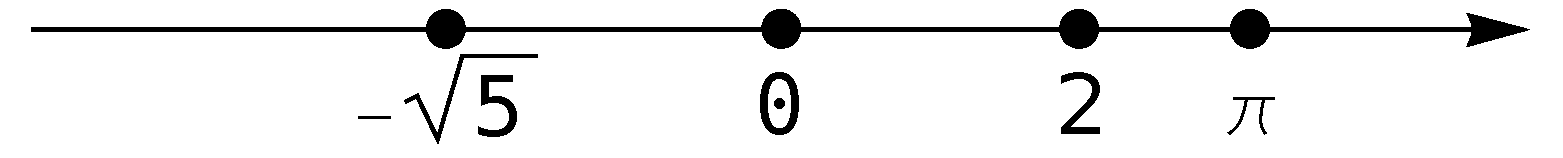
\includegraphics[width=0.4\textwidth]{fig_sets_7}
\end{center}
With every real number $x$ corresponds one point on this line, and vice versa, every point on this line represents one real number. This line is called the \textbf{real number line} (\textit{re\"ele getallenas}). \index{real number line}\index[aut]{re\"ele getallenas}


In addition to the set of real numbers, we often make reference to one of the following subsets for the sake of brevity:
\begin{eqnarray*}
	\mathbb{R}_0 &=& \mathbb{R} \backslash \{0\},\\
	\mathbb{R}^+ &=& \{x\; |\; x\in \mathbb{R} \;\wedge\; x \geq 0\},\\
	\mathbb{R}^- &=& \{x\; |\; x\in \mathbb{R} \;\wedge\; x \leq 0\},\\
	\mathbb{R}^+_0 &=& \{ x\; |\; x\in \mathbb{R}\;\wedge\; x > 0 \},\\
	\mathbb{R}^-_0 &=& \{ x\; |\; x\in \mathbb{R}\;\wedge\; x < 0 \}.\\
\end{eqnarray*}

Moreover, it is possible to extend $\mathbb{R}$ with two more elements, namely positive infinity ($+\infty$) and negative infinity  ($-\infty$), which are defined as:
$$ 
\forall x\in\mathbb{R}:\quad-\infty<x<+\infty\,,
$$
and which do not belong to $\mathbb{R}$. Doing so, one arrives at the set of \textbf{extended real numbers} (\textit{uitgebreide re\"ele getallen}):
$$
\overline{\mathbb{R}}=\mathbb{R}\cup\left\{-\infty,+\infty\right\}.
$$


For completeness, it should be mentioned that there is a further extension of the set of real numbers possible to the set of \textbf{complex numbers} (\textit{complexe getallen})\index{complex number}\index[aut]{complex getal}\index{number ! complex}\index[aut]{getal ! complex}, defined by 
$$\mathbb C=\left\{a+i\,b \, \mid \, \left(a,b  \in \mathbb R\right) \, \wedge \, \left(i^2=-1\right) \right\}\,.$$
%$$\mathbb C=\left\{a+i\,b \, \mid \, a,b  \in \mathbb R \, \wedge \, i=\sqrt{-1} \right\}.$$
This extension allows us, for instance, to compute the square root of a negative number. The complex numbers are discussed in Section~\ref{sec_complex}. Throughout this course we will, however, mostly restrict our discussion to the set of real numbers. 

\ifanalysis
\begin{remark}[History of complex numbers]
	A long history preceded the development of the set of complex numbers. Three milestones are listed below.
	\begin{enumerate}
		\item Negative numbers
		\begin{itemize}
			\item China (202 BC -- AD 220): \textit{Nine Chapters on the Mathematical Art (Jiu zhang suan-shu)}
			\item Red counting rods were used to denote gains (positive coefficients) and black rods for losses (negative).
		\end{itemize}
		\item The number $0$
		\begin{itemize}
			\item Ancient civilisations such as the Greeks and Romans had no real concept of zero as a number, although the Babylonians left blanks.
			\item ca. 650 AD : Indian mathematics introduced 0, which was eventually spread to the Arab and Asian nations.
			\item In Europe 0 was introduced (along with the rest of the Hindu-Arabic number system) mainly via the \textit{Liber Abaci} by Fibonacci. Initially, there was a strong opposition against new numeric system by people clinging on the old Roman system.
		\end{itemize} 
		\item The number $i$
		\begin{itemize}
			\item Italy, 16th century: Studied during the discovery of algebraic solutions for the roots of cubic and quartic polynomials by Italian mathematicians
		\end{itemize}
	\end{enumerate}
\end{remark}
\fi



\subsection{Real number arithmetic}
\label{sec_real_number}
\subsubsection{Addition and multiplication}
In the set of real numbers, we can define to main operations namely, addition ($+$) and multiplication ($\cdot$). If $a, b$ and $c$ are three real numbers, we have the following five axioms:

\index{commutativity}\index[aut]{commutativiteit}\index{associativity}\index[aut]{associativiteit}
\begin{enumerate}
	\item \textbf{Algebraic closure} (\textit{algebra\"isch gesloten}):
	\begin{align*}
	a+b\in \mathbb{R} \quad & \mbox{ and }\quad a\cdot b \in\mathbb{R}\,.\\
	\intertext{\item  \textbf{Commutativity} (\textit{commutativiteit}):}
	a+b=b+a \quad & \mbox{ and }\quad a\cdot b=b\cdot a\,.\\
	\intertext{\item \textbf{Associativity} (\textit{associativiteit}):}
	a+(b+c)=(a+b) +c \quad & \mbox{ and }\quad a\cdot(b\cdot c)=(a\cdot b)\cdot c\,.\\
	\intertext{\item \textbf{Identity property}:}
	a+0=0+a=a \quad & \mbox{ and }\quad a\cdot1=1\cdot a=a\,.\\
	\intertext{\item \textbf{Inverse property}:}
	a+(-a)=(-a)+a=0 \quad & \mbox{ and }\quad a\cdot a^{-1}=a^{-1}\cdot a=1\\
	\end{align*}
\end{enumerate}

Essentially, the identity property indicates that 0 is the \textbf{neutral element} (\textit{neutraal element})  of the addition operation and 1 is neutral element of the multiplication operation, while the inverse property shows that there is always an \textbf{opposite element} (\textit{tegengesteld element})  in the case of addition and an \textbf{inverse element}  (\textit{invers element}) in the case of multiplication. Finally, according to the sixth axiom of real numbers, multiplication \textbf{distributes} over addition:\index{distributivity}\index[aut]{distributiviteit}
$$
a\cdot (b+c) = a\cdot b + a\cdot c \quad\mbox{ and }\quad(a+b)\cdot c = a\cdot c + b\cdot c\,. 
$$ 
The operations of subtraction and division are not listed above because they fail to  possess  many  of  the aforementioned  properties.  More precisely, subtraction   and   division   are   not   commutative, nor associative, as for instance $4-1\neq1-4$ and likewise $(4-1)-2\neq4-(1-2)$. \index{neutral element}\index[aut]{neutraal element}\index{inverse element}\index[aut]{invers element}\index{opposite}\index[aut]{tegengestelde}

\ifanalysis

	Since any set  that has the operations of addition and multiplication
	defined on it and that satisfies the preceding axioms is called a \textbf{field} (\textit{veld}), the sets of rational and real numbers constitute fields.  On the other hand, the set of integers is not a field, as it does not contain multiplicative inverses. For example, there is no $x\in\mathbb{Z}$ such that $2x=1$.
	
	Clearly, we may extend the notion of a field to an \textbf{ordered field} (\textit{geordend veld}) if the underlying set is ordered. Hence, the sets of rational and real numbers are ordered fields.
	\index{field}
	\index[aut]{veld}

\fi

Throughout this course we will sometimes be confronted with problems involving the summation\index{summation}\index[aut]{sommatie} of many numbers, e.g.
$$
a_0+a_1+a_2+\cdots+a_n\,,
$$
where $n$ is some natural number. Clearly, writing such sums can become quite cumbersome, so a shorthand notation thereof has been established using the \textbf{capital sigma notation}\index[aut]{sommatie!hoofdletter sigma notatie}; that is

$$
a_0+a_1+a_2+\cdots+a_n=\displaystyle\sum_{i=0}^na_i\,,
$$
where $i$ is the \textbf{summation index}  (\textit{index})\index{summation!summation index}\index[aut]{sommatie!index} and $a_i$ is a \textbf{generic term}  (\textit{algemene term})\index{sommatie!generic term}\index[aut]{sommatie!algemene term} in the summation. This expression should be read as the sum of the numbers $a_i$ for $i$ going from 0 to $n$. Here, the index $i$ starts at 0, but this is not a requisite. 

We can formulate the following useful properties of summations:
\begin{itemize}
	\item Sum or difference of summations:
	$$
	\displaystyle\sum_{i=0}^n a_i\pm \displaystyle\sum_{i=0}^nb_i=\displaystyle\sum_{i=0}^n\left(a_i\pm b_i\right)\,.
	$$
	\item Splitting a summation:
	$$
	\displaystyle\sum_{i=0}^n a_i=\displaystyle\sum_{i=0}^m a_i+\displaystyle\sum_{i=m+1}^n a_i\,,\, \text{where } m<n\,.
	$$
	\item Scalar multiplication:
	$$
	c\cdot \displaystyle\sum_{i=0}^n a_i=\displaystyle\sum_{i=0}^n c\cdot a_i\,, \text{where}\, c\in\mathbb{R}\,.
	$$
	\item Constant summation:
	$$
	\displaystyle\sum_{i=0}^n c=c\cdot(n+1)\,, \text{where}\, c\in\mathbb{R}\,. 
	$$
	
\end{itemize}

Moreover, we recall (without proof) two useful identities, that will be used in later chapters and involve the sum of the first $n$ (squared) natural numbers:
\begin{equation}
\displaystyle\sum_{i=1}^n i = \dfrac{n(n+1)}{2}\qquad\text{and}\qquad\displaystyle\sum_{i=1}^n i^2 = \dfrac{n(n+1)(2n+1)}{6}.
\label{thm:summation}
\end{equation}

% BIOIR: meervoudige sommatie en vermenigvuldiging van sommen (ins: wiskundige basisvaardigheden)

Similarly to the capital sigma notation for summation, we can use the \textbf{capital pi notation}\index{capital pi notation}\index[aut]{hoofdletter pi notatie} for the product of $n$ numbers:
$$
\displaystyle\prod_{i=0}^n a_i=a_0\cdot a_1\cdot a_2\cdots a_n\,. 
$$

Using the capital pi notation, it becomes easy to define the so-called \textbf{factorial} (\textit{faculteit}) of a natural number $n$, denoted $n!$:
$$
n!=\prod\limits_{k=1}^{n}k=1\cdot 2\cdot 3\cdot \ldots \cdot n.
$$

From here on, we will mostly drop the dot-notation to denote multiplication and use a blank space instead. Only in case of ambiguity (e.g.\ when multiplying two numbers), we will hold on the dot-notation for clarity.

\subsubsection{Exponentiation}

In addition to the four elementary operations in $\mathbb{R}$, namely addition, subtraction, multiplication and division, we can also define \textbf{exponentiation}  (\textit{machtsverheffing}). It involves two numbers, the \textbf{base}  (\textit{grondtal}) $b\in\mathbb{R}_0$ and the \textbf{exponent} (\textit{exponent}) $n$ and is written as $b^n$. When $n$ is a strictly positive integer, exponentiation corresponds to repeated multiplication of the base: that is, $b^n$ is the product of multiplying $n$ bases:\index{exponentiation}\index[aut]{machtsverheffing}\index{base}\index[aut]{basis}\index{exponent}\index[aut]{macht}
$$
b^n=\underbrace{b\, b\, b\,\cdots\,b}_{n \text{ factors}}\,.
$$
This expression should be read as $b$ raised to the power of $n$. For negative powers, we have
$$
b^{-n}=\dfrac{1}{b^n}\,.
$$
By convention, it holds that any non-zero number raised to the 0 power is 1, i.e. $b^0=1$ if $b\neq0$. The expression $b^2$ is often  called the square of $b$ or $b$ squared, while $b^3$ is frequently called the cube of $b$ or $b$ cubed.

The exponent does not necessarily have to be an integer, it can as well be a rational number, such as $1/n$, where $n\in\mathbb{N}_0$. More precisely, we can have
$$
x=b^{\frac{1}{n}}\,,
$$
which should be interpreted as the number $x$ for which the $n$-th power equals $b$. This implies that $b^{1/n}$ is a solution to the equation
$$
x^n=b\,. 
$$

\ifcalculus
\begin{example}
	Moore's law concerns the observation that the number of transistors in a dense integrated circuit doubles about every two years. The observation is named after Gordon Moore, whose 1965 paper described a doubling every year in the number of components per integrated circuit, and projected this rate of growth would continue for at least another decade. Mathematically, we can state this law as
	$$
	P_n=P_0\,2^n\,,
	$$
	where $P_0$ [--] is the number of transistors in some reference year, $n$ [--] the number of two-year periods, and $P_n$ [--] the number transistors $n$ two-year periods passed the reference year. In 1988, the number of transistors in the Intel 386 SX microprocessor was 275 000. What were the transistors counts of the Pentium II Intel microprocessor in 1997? 
	
	\xhrulefill{gray}{2.5pt}Solution \xhrulefill{gray}{2.5pt}
	
	Between 1988 and 1997 there are 9 years, so 4.5 periods of two years. Hence, if Intel doubles the number of transistors every two years, the new processor would have
	\begin{eqnarray*}
		P_{9/2} = 275\,000 \cdot 2^{\frac{9}{2}}
		= 275\,000 \cdot 22.63
		= 6\,223\,250  
	\end{eqnarray*}
	transistors in 1997. In fact, in 1997, the Pentium II had 7.5 million transistors (Figure~\ref{fig_sets_8}). In other words, since 1988 up until 1997, Intel had been doubling the number of transistors in its microprocessors in less than every two years.
	
	\begin{figure}[H]
		\begin{center}
			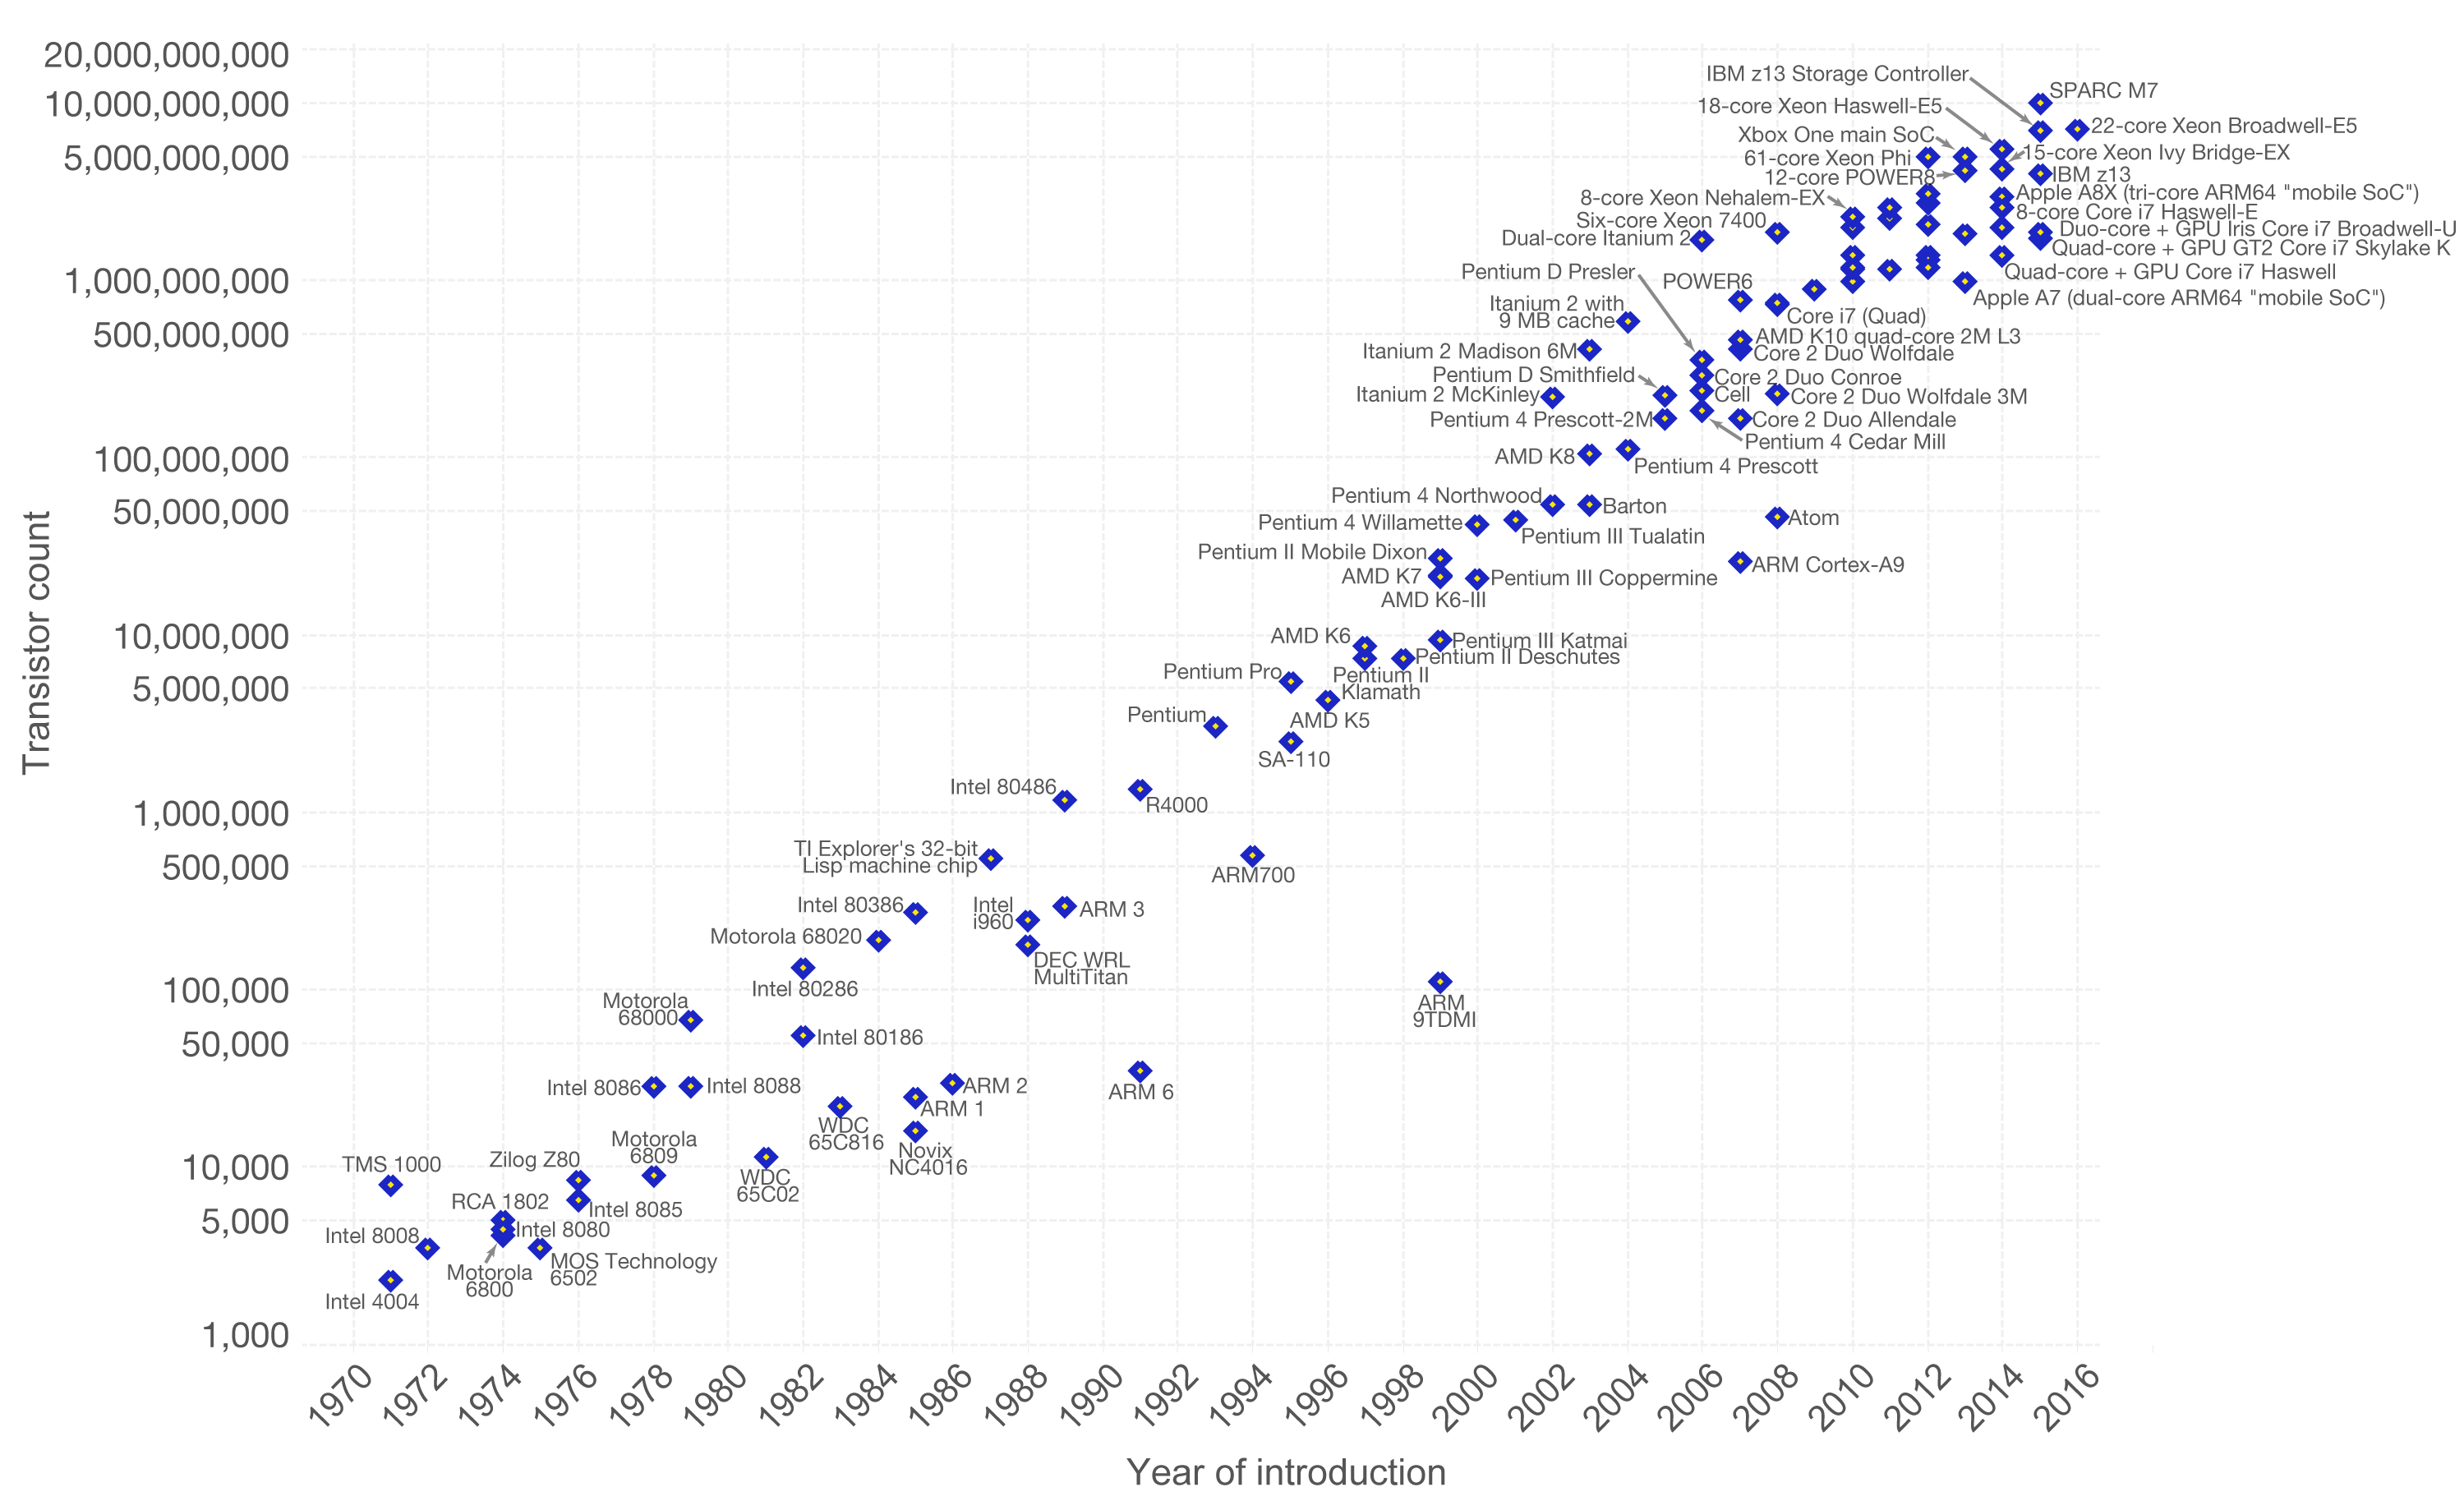
\includegraphics[width=0.75\textwidth]{fig_sets_8}
			\caption{Number of transistors in computer hardware manufactured since 1970.}
			\label{fig_sets_8}
		\end{center}
	\end{figure}
	
	
\end{example}
\fi

Alternatively, $b^{1/n}$ is often written using the radical symbol as $\sqrt[n]{b}$. It is called the principal $n$-th root of $b$. If $n$ is even and $b$ is positive, then $x^n = b$ has two real solutions because even powers of real numbers are always positive. These solutions are the positive and negative $n$-th roots, i.e.
$$
\sqrt[n]{a}\qquad \mbox{ and }\qquad -\sqrt[n]{a}\,. 
$$
If $b$ is negative, the equation has no solution in the set real numbers for even $n$. On the other hand, if $n$ is odd, then $x^n = b$ has exactly one real solution $b^{1/n}$ that is positive if $b$ is positive and negative if $b$ is negative. Finally, taking a positive real number $b$ to a rational exponent $m/n$, where $m$ is an integer and $n$ is a positive integer, and considering principal roots only, yields
$$
b^{\frac{m}{n}}=\left(b^m\right)^{\frac{1}{n}}=\sqrt[n]{b^m}=\left(\sqrt[n]{b}\right)^m\,.
$$

The following basic identities hold for the operation of exponentiation for every $a,b\in\mathbb{R}$ and $p,q\in\mathbb{Q}$:
\begin{itemize}
	\item $a^p\, a^q=a^{p+q}\,,$
	\item $\left(a^p\right)^q=a^{p\, q}\,,$
	\item $\left(a\, b\right)^p=a^p\, b^p\,,$
\end{itemize}
and recalling that $1/a^p=a^{-p}$, we also have:
\begin{itemize}
	\item $\dfrac{a^p}{a^q}=a^{p-q}\,,\qquad$ if $a\neq 0$\,,
	\item $\left(\dfrac{a}{b}\right)^p=\dfrac{a^p}{b^p}\,,\qquad$ if $b\neq 0$\,.
\end{itemize}
However, be aware that exponentiation is not commutative, nor associative, unlike addition and multiplication. Indeed, it is clear that $2^3=8\neq3^2=9$ and likewise 
$$
\left(2^3\right)^4=8^4=4096\neq 2^{(3^4)}=2^{81}=2417851639229258349412352\,.
$$


\begin{example}
	Yearly, there are about three consecutive generations of box moths in Belgium. Suppose the number of box moths (\textit{Cydalima perspectalis}) in generation $i$ can be described as follows:
	$$
	B_{i}=r\,B_{i-1}\,,
	$$
	where $r$ [T$^{-1}$] represents the growth rate of the box moth population. Assuming that we know the initial number of box moths (generation 0), we can compute the number of box moths in generation 1 as
	$$
	B_1=r\,B_0\,.
	$$
	Then, we can compute the number of box moths in generation 2:
	$$
	B_2=r\,B_1=r\,r\,B_0=r^2\,B_0\,,
	$$
	and so on. 
	
	The total number of box moths that has seen daylight up to and including generation $n$, can then be written as
	\begin{eqnarray*}
		T_n&=&\displaystyle\sum_{i=0}^nB_i\,,\\
		&=&B_0+B_1+B_2+\cdots+B_n\,,\\
		&=&B_0+r\,B_0+r^2\,B_0+\cdots+r^n\,B_0\,.
	\end{eqnarray*}
	For instance, if $B_0=5$, $r=1.1$ and $n=5$, we find $T_5\approx39$ individuals. 
\end{example}

For what concerns the square and cube of the sum and difference of two real numbers, we can infer the following well-known identities:\index[aut]{merkwaardige producten}
\allowdisplaybreaks
\begin{eqnarray*}
	(a+b)^2&=&a^2+2ab+b^2\\ 
	(a-b)^2&=&a^2-2ab+b^2\\
	(a+b)(a-b)&=&a^2-b^2\\
	(a+b)^3&=&a^3+3a^2b+3ab^2+b^3\\
	(a-b)^3&=&a^3-3a^2b+3ab^2-b^3\\
	(a+b)(a^2-ab+b^2)&=&a^3+b^3\\
	(a-b)(a^2+ab+b^2)&=&a^3-b^3\\
\end{eqnarray*}

\subsubsection{Arithmetic in $\overline{\mathbb{R}}$}
Obviously, the rules of arithmetic that apply to $\mathbb{R}$ apply to $\overline{\mathbb{R}}$ as well, but we need to introduce a few more rules involving a real number $a\in\mathbb{R}$ and/or $+\infty$ and/or $-\infty$. With regard to addition, we have
\begin{align*}
a+(+\infty) \quad&=\quad (+\infty)+ a\quad=\quad+ \infty\,,\\ 
a+(-\infty)\quad&=\quad(-\infty) + a\quad=\quad- \infty\,,\\
(+\infty)+(+\infty)\quad&=\quad+\infty\,,\\
(-\infty)+(-\infty)\quad&=\quad-\infty\,,\\
\intertext{while for subtraction we have}
a-(+\infty) \quad&=\quad - \infty\,,\\
a-(-\infty) \quad&=\quad + \infty\,,\\
(+\infty) - a \quad&=\quad + \infty\,,\\
(-\infty) - a \quad&=\quad - \infty\,,\\
(+\infty)-(-\infty) \quad&=\quad +\infty\,,\\
(-\infty)-(+\infty) \quad&=\quad -\infty\,.
\end{align*}

For multiplication, we accordingly have (considering $a\in\mathbb{R}_0$)
$$
a\cdot(+\infty)=(+\infty)\cdot a=\left\{\begin{array}{lcl}
+\infty\,,&\mbox{ if }&a>0\,,\\
-\infty\,,&\mbox{ if }&a<0\,,\end{array}\right.
$$
and 
$$
a\cdot(-\infty)=(-\infty)\cdot a=\left\{\begin{array}{lcl}
-\infty\,,&\mbox{ if }&a>0\,,\\
+\infty\,,&\mbox{ if }&a<0\,.\end{array}\right.
$$
Likewise, for products involving $+\infty$ and/or $-\infty$ only:
\begin{eqnarray*}
	(+\infty)\cdot(+\infty)&=&+\infty\,,\\
	(-\infty)\cdot(-\infty)&=&+\infty\,,\\
	(+\infty)\cdot(-\infty)&=&(-\infty).(+\infty)\; \; =\; \; -\infty\,.
\end{eqnarray*}

And for the division, we have
$$
\dfrac{a}{+\infty} = \dfrac{a}{-\infty} = 0\,,
$$
irrespective of the sign of $a\in\mathbb{R}_0$, and
%$$
%\dfrac{a}{0}=\left\{\begin{array}{lcl}
%+\infty\,,&\mbox{ if }&a>0\,,\\
%-\infty\,,&\mbox{ if }&a<0\,,\end{array}\right.
%$$
$$
\dfrac{+\infty}{a}=\left\{\begin{array}{lcl}
+\infty\,,&\mbox{ if }&a>0\,,\\
-\infty\,,&\mbox{ if }&a<0\,,\end{array}\right.
$$
%and finally
$$
\dfrac{-\infty}{a}=\left\{\begin{array}{lcl}
-\infty\,,&\mbox{ if }&a>0\,,\\
+\infty\,,&\mbox{ if }&a<0\,.\end{array}\right.
$$
%For what concerns exponentiation, we have 
%$$
%a^{+\infty}=\left\{\begin{array}{lcl}
%+\infty\,,&\mbox{ if }&a>1\,,\\
%1\,,&\mbox{ if }&a=1\,,\\
%0\,,&\mbox{ if }&-1<a<1\,,\end{array}\right.
%$$
%
%and
%$$
%a^{-\infty}=\left\{\begin{array}{lcl}
%0\,,&\mbox{ if }&a>1\,,\\
%+\infty\,,&\mbox{ if }&-1<a<1\,,\\
%0\,,&\mbox{ if }&a<-1\,.\end{array}\right.
%$$

And finally, for what concerns principal $n$-th roots, for $n\in\mathbb{N}_0$:
\begin{eqnarray*}
	\sqrt[n]{+\infty}&=&+\infty\,,\\
	\sqrt[2n+1]{-\infty}&=&-\infty\,.
\end{eqnarray*}

\ifcourse
\ifanalysis

	\subsection{Completeness of $\mathbb{R}$}
	We have already seen that the set of real numbers is an ordered field. Even more important is that this ordered field is in fact the
	only complete ordered field. Basically, this means that if an alien were to construct a mathematical system on the basis of Axioms (1)-(6) from Section~\ref{sec_real_number} endowed with an ordering and satisfying the least-upper-bound-property (Definition~\ref{defn:lub}), the alien's system would differ from the real number system we devised only in that the alien might use different symbols for the real numbers and $+$, $\cdot$ and $<$.
	
	This all gives rise to the following intuitive theorem. 
	
	\begin{theorem}[Supremum]\label{thmtype:1.1.3}
		If a nonempty set $S$ of real numbers  is bounded above, then
		$\sup S$ is the unique real number $\beta$ such that
		\begin{enumerate}
			\item  $x\leq\beta$ for all $x$ in $S;$
			\item  if $\epsilon>0$ (no matter how small), there is an $x_0$ in
			$S$ such that $x_0>\beta-\epsilon.$
		\end{enumerate}
	\end{theorem}
	Essentially, this theorem can be  interpreted geometrically as follows: $\beta$ is the supremum of $S$ if no point of $S$ is to the right of $\beta$, but there is at least one point of $S$ to the right of any number less than $\beta$. 
	
	\begin{proof}
	To prove the theorem, we first show that $\beta=\sup S$ has properties 1) and
	2). Since $\beta$ is an upper bound of $S$, it must satisfy
	1). Since any real number $a$ less than $\beta$ can be written
	as $\beta-\epsilon$ with $\epsilon=\beta-a>0$, 2) is just
	another way of saying that no number less than $\beta$ is an upper
	bound of $S$. Hence, $\beta=\sup S$ satisfies 1) and 2).
	
	Now we show that there cannot be more than one real number with
	properties 1) and 2). Suppose that $\beta_1<\beta_2$ and
	$\beta_2$ has property 2); thus, if $\epsilon>0$, there is an
	$x_0$ in $S$ such that $x_0>\beta_2-\epsilon$. Then, by taking
	$\epsilon=\beta_2-\beta_1$, we see that there is an $x_0$ in $S$ such
	that
	$$
	x_0>\beta_2-(\beta_2-\beta_1)=\beta_1,
	$$
	so  $\beta_1$ cannot have property 1). Therefore, there cannot
	be more than one real number that satisfies both 1) and
	2).
	\end{proof}
	
	Obviously, we can state a similar theorem for what concerns the infimum.
	\\
	
	\begin{theorem}[Infimum]\label{thmtype:1.1.8}
		If a nonempty set $S$ of real numbers  is bounded below$,$ then
		$\inf S$ is the unique real number $\alpha$ such that
		\begin{enumerate}
			\item % \part{a}
			$x\ge\alpha$ for all $x$ in $S;$
			\item % (b)
			if $\epsilon>0$ $($no matter how small$\,)$, there is an $x_0$ in $S$
			such that
			$x_0<
			\alpha+\epsilon.$
		\end{enumerate}
	\end{theorem}
 \begin{proof}
 As above.
 \end{proof}
	
	
	
	
	
	The real numbers also have the property that it is possible to exceed any positive number, no matter how large, by adding an arbitrary positive number, no matter how small, to itself sufficiently many times.
	
	
	
	\begin{theorem}[Archimedean property]
		\label{thmtype:1.1.4}
		If $\rho$ and $\epsilon$ are positive$,$ then $n\epsilon>\rho$ for
		some $n\in\mathbb{N}_0$.
	\end{theorem}
\begin{proof}	
	The proof of this theorem is by contradiction.
	If the statement is false, $\rho$ is an upper bound of
	the set
	$$
	S=\set{x},
	$$
	where $x=n\epsilon$ and $n\in\mathbb{N}_0$. Therefore, since the set of real numbers is complete, $S$  has a supremum $\beta$ and it holds that 
	\begin{equation}\label{eq:1.1.9}
	n\epsilon\le\beta, 
	\end{equation}
	for all $n\in\mathbb{N}_0$.
	Since $n+1$ is in $\mathbb{N}_0$ whenever $n$ is, Equation~\eqref{eq:1.1.9} implies that
	$$
	(n+1)\epsilon\leq\beta
	$$
	and therefore
	$$
	n\epsilon\leq\beta-\epsilon
	$$
	for all $n\in\mathbb{N}_0$. Hence,
	$\beta-\epsilon$ is an upper bound of $S$.  Since $\beta-\epsilon
	<\beta$, this contradicts the definition of~$\beta$.
\end{proof}	
	

\fi
\fi


\subsection{Intervals in $\mathbb{R}$}
\label{intervals}
Segments of the real number line are called \textbf{intervals} (\textit{interval}) of numbers.  Table~\ref{tab_sets_1} gives a summary of the interval notation for real numbers.  
If the endpoint is included in the interval, we use closing square brackets, `$[$' or `$]$', when defining the interval and use a filled dot to indicate membership in the interval on the real number line. Otherwise, we use opening square brackets, `$]$' or `$[$', and a circle to indicate that the endpoint is not part of the set.  If the interval does not have finite endpoints, we use the symbols $-\infty$ to indicate that the interval extends infinitely to the left and $+\infty$ to indicate that the interval extends infinitely to the right.  Since infinity is a concept, and not a number, we always use opening square brackets when using these symbols in interval notation.%, and use an appropriate arrow to indicate that the interval extends infinitely in one (or both) directions.

It should not be forgotten that any interval in $\mathbb{R}$ corresponds with a certain set of real numbers, so that we may apply the set operations introduced in Section~\ref{setoperations} directly to intervals. For example,  if $A = [-5,3\left[\right.$ and $B = \left.\right]1, +\infty\left[\right.$, then we easily find $A \cap B = \left.\right]1,3\left[\right.$ and   $A \cup B = [-5,+\infty\left[\right.$. Likewise, we find $A\setminus B=[-5,1]$. 


\begin{table}[t]
	\caption{Interval notation for two real numbers $a$ and $b$ for which it holds that $a<b$. }
	\label{tab_sets_1}
	\begin{center}
		\renewcommand{\arraystretch}{2}%
		\begin{tabular}{c|c|c} 
			
			Set of real numbers & Interval notation &  Region on the real number line  \\
			\hline\hline
			
			&  & \\
			\shortstack{$\{x\,|\,a<x<b\}$ \\ \hfill}& \shortstack{$\left.\right]a,b\left[\right.$ \\ \hfill} & 
			
			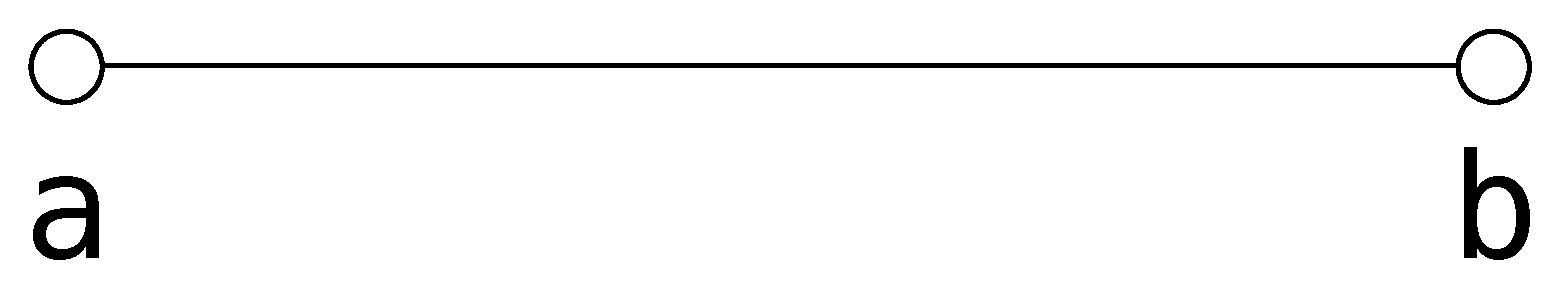
\includegraphics[width=0.25\textwidth]{fig_sets_9a}  \\ \hline
			
			& &  \\
			\shortstack{$\{x\,|\,a\leq x<b\}$ \\ \hfill}& \shortstack{$[a,b\left[\right.$ \\ \hfill} & 
			
			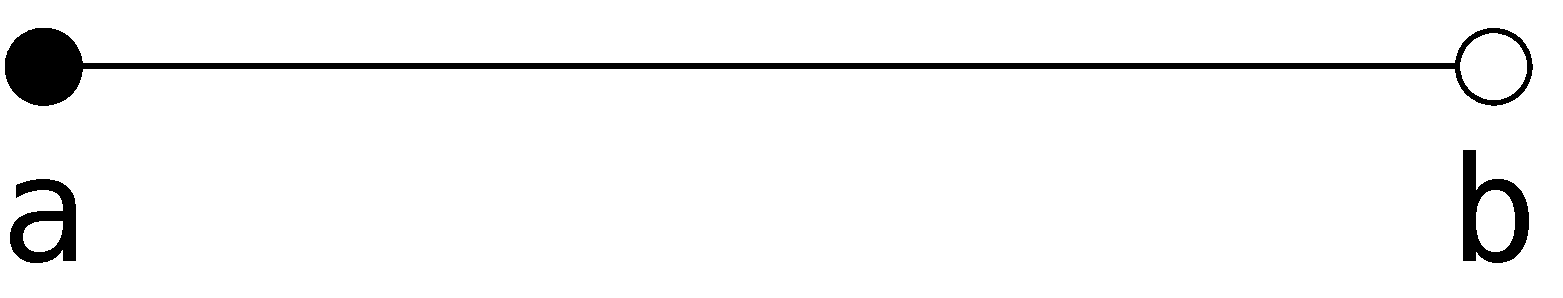
\includegraphics[width=0.25\textwidth]{fig_sets_9b}  \\
			\hline
			
			&  & \\
			\shortstack{$\{x\,|\,a<x\leq b\}$ \\ \hfill}&\shortstack{$\left.\right]a,b]$ \\ \hfill} & 
			
			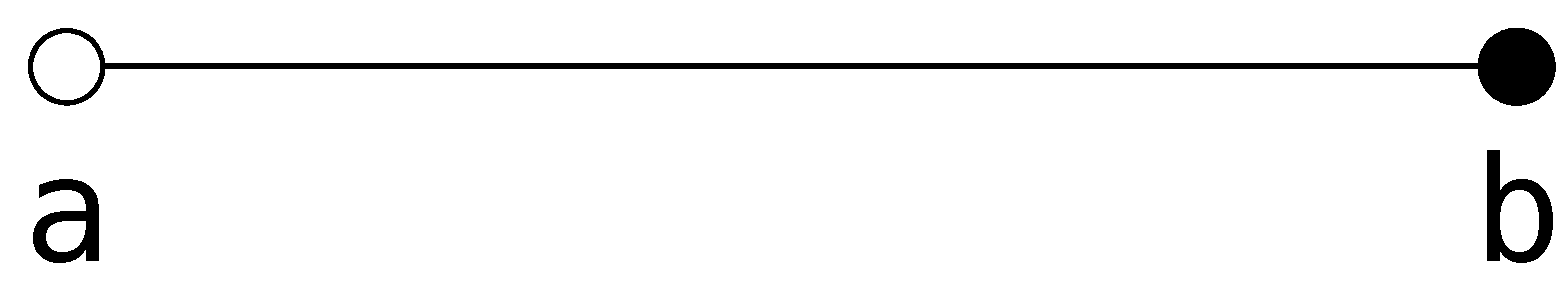
\includegraphics[width=0.25\textwidth]{fig_sets_9c}  \\
			\hline
			
			&  & \\
			\shortstack{$\{x\,|\,a\leq x \leq b\}$ \\ \hfill}& \shortstack{$[a,b]$ \\ \hfill}& 
			
			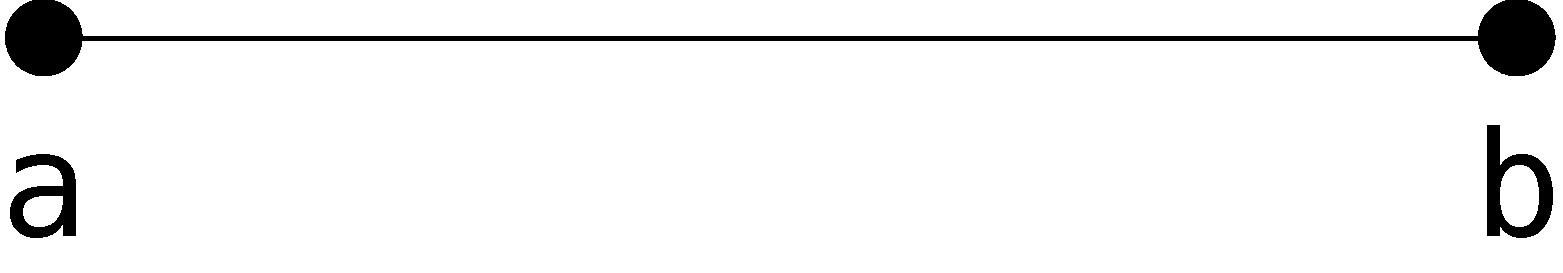
\includegraphics[width=0.25\textwidth]{fig_sets_9d}   \\
			\hline
			
			& & \\
			\shortstack{$\{x\,| \, x<b\}$ \\ \hfill}& \shortstack{$\left.\right]-\infty,b\left[\right.$ \\ \hfill}& 
			
			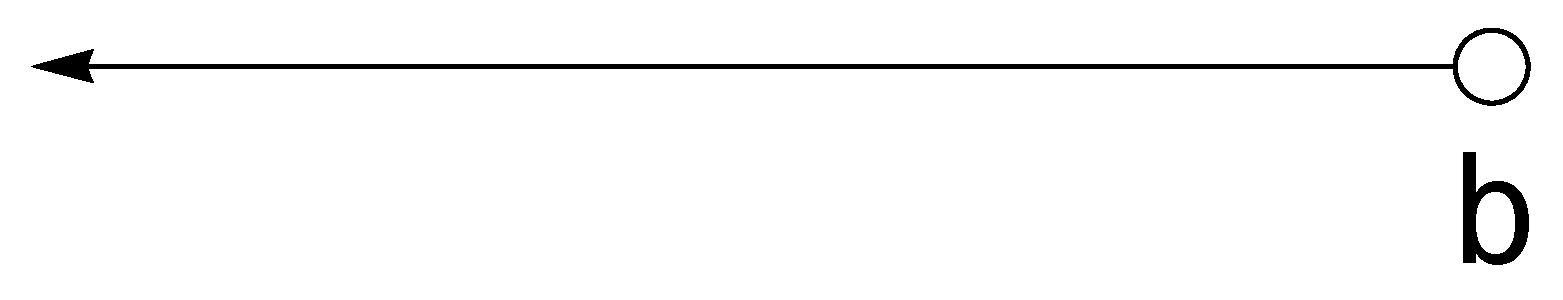
\includegraphics[width=0.25\textwidth]{fig_sets_9e}  \\
			\hline
			
			
			&  & \\
			
			\shortstack{$\{x\,| \, x \leq b\}$ \\ \hfill} & \shortstack{$\left.\right]-\infty,b]$ \\ \hfill}& 
			
			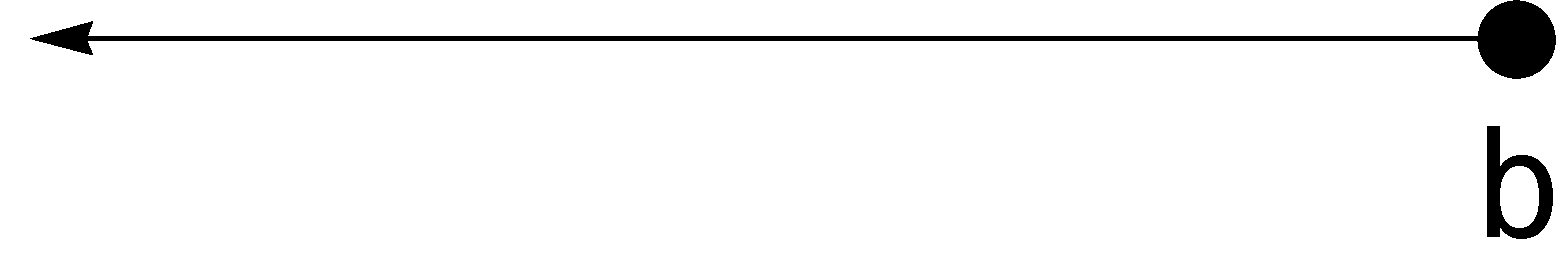
\includegraphics[width=0.25\textwidth]{fig_sets_9f}    \\
			\hline
			
			&  & \\
			\shortstack{$\{x\,| \, x>a\}$ \\ \hfill}& \shortstack{$\left.\right]a,+\infty\left[\right.$ \\ \hfill}& 
			
			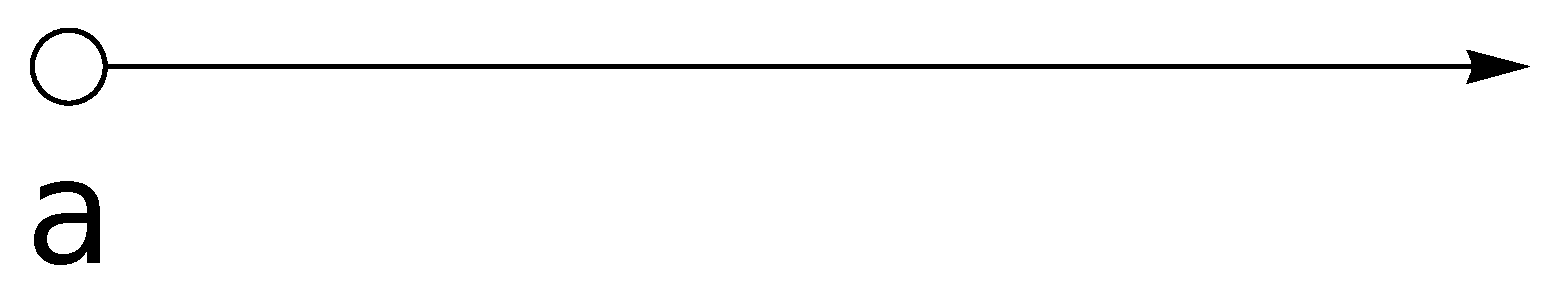
\includegraphics[width=0.25\textwidth]{fig_sets_9g}   \\
			\hline
			
			&  & \\
			\shortstack{$\{x\,| \, x \geq a \}$ \\ \hfill}& \shortstack{$[a,+\infty\left[\right.$ \\ \hfill} & 
			
			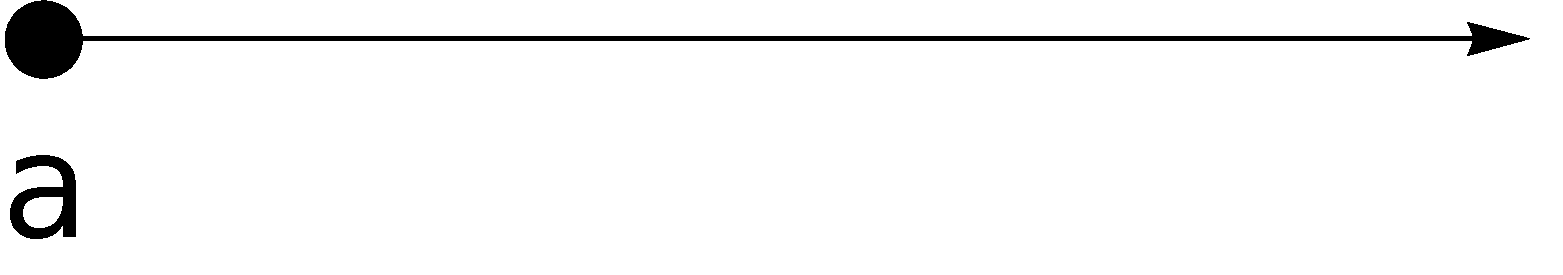
\includegraphics[width=0.25\textwidth]{fig_sets_9h}   \\
			\hline
			
			&  & \\
			\shortstack{$\mathbb R$ \\ \hfill}& \shortstack{$\left.\right]-\infty,+\infty\left[\right.$ \\ \hfill} & 
			
			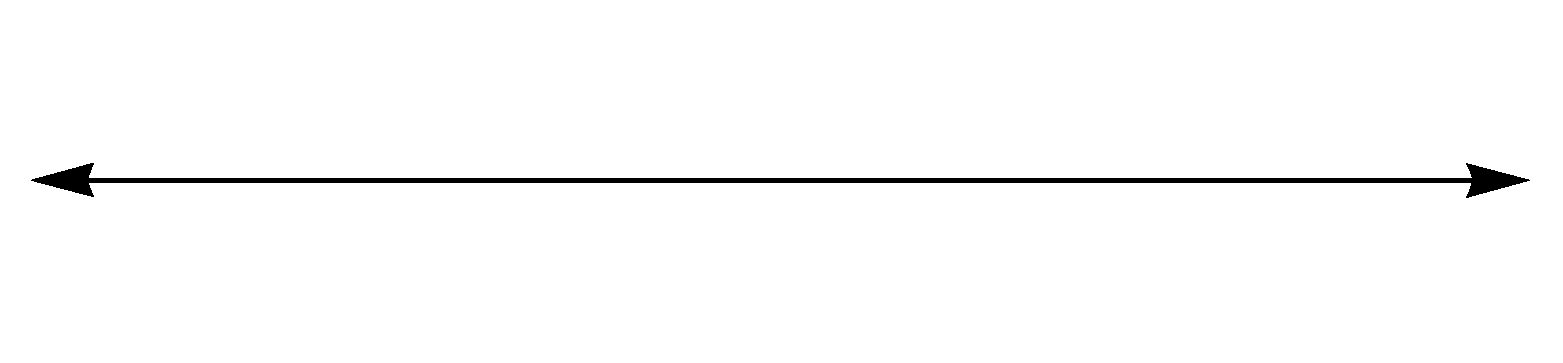
\includegraphics[width=0.25\textwidth]{fig_sets_9i}  \\
			
			
		\end{tabular}
		
	\end{center}
\end{table}



\ifcalculus
\begin{example} \label{unionex} 
	Express the following sets of numbers using interval notation.
	
	\begin{multicols}{2}
		
		\begin{enumerate}
			
			\item  $\{ x \, | \, x \leq -2 \, \, \vee \, \,  x \geq 2 \}$
			
			
			
			
			%\end{enumerate}
			
			%\end{multicols}
			
			%\begin{multicols}{2}
			
			%\begin{enumerate}
			
			
			\item  $\{ x \, | \, x \neq \pm 3 \}$
			
			\item  $\{ x \, | \, -1 < x \leq 3 \,\, \vee \,\, x = 5\}$
			
		\end{enumerate}
		
	\end{multicols}
	
	\xhrulefill{gray}{2.5pt}Solution \xhrulefill{gray}{2.5pt}
	
	\begin{enumerate}
		
		\item  The best way to proceed here is to graph the set of numbers on the number line.  The inequality $x \leq -2$ corresponds to the interval $\left.\right]-\infty, -2]$ and the inequality $x \geq 2$ corresponds to the interval $[2, +\infty\left[\right.$.  Since we are looking to describe the real numbers $x$ in one of these or the other, we have $\{ x \, | \, x \leq -2 \, \, \vee \, \,  x \geq 2 \} = \left.\right]-\infty, -2] \cup [2, +\infty\left[\right.$.
		
		\begin{center}
			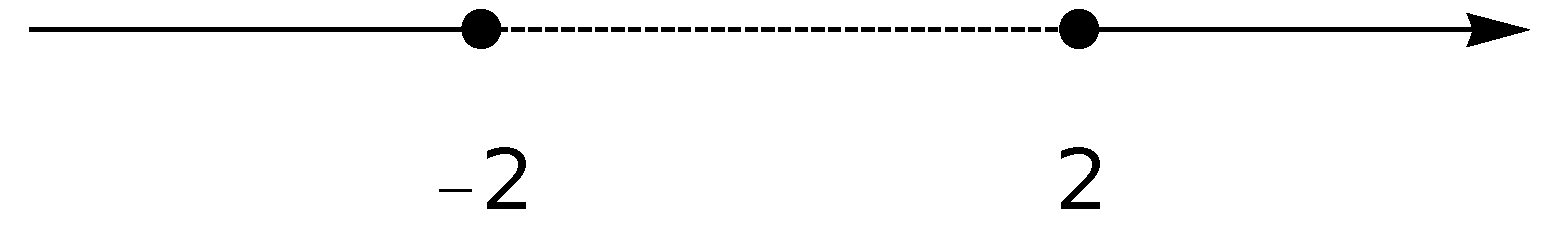
\includegraphics[width=0.4\textwidth]{fig_sets_10a}
		\end{center}
		
		
		
		\item  For the set $\{ x \, | \, x \neq \pm 3 \}$, we exclude both $x=3$ and $x=-3$ from our set.  This breaks the number line into three intervals, $\left.\right]-\infty, -3\left[\right.$, $\left.\right]-3,3\left[\right.$ and $\left.\right]3, +\infty\left[\right.$, so $\{ x \, | \, x \neq \pm 3 \} = \left.\right]-\infty, -3\left[\right. \cup \left.\right]-3,3\left[\right. \cup \left.\right]3, +\infty\left[\right.$.
		
		
		\begin{center}
			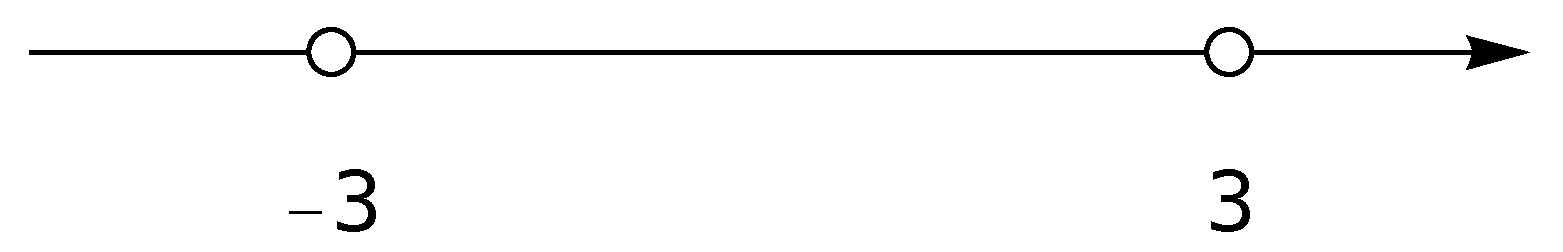
\includegraphics[width=0.4\textwidth]{fig_sets_10b}
		\end{center}
		
		
		\item  Graphing the set $\{ x \, | \, -1 < x \leq 3 \,\, \vee \,\, x = 5\}$, we get one interval, $\left.\right]-1,3]$ along with a single number, or point, $\{ 5\}$.
		Consequently, we have $\{ x \, | \, -1 < x \leq 3 \,\, \vee \,\, x = 5\} = \left.\right]-1,3] \cup \{ 5\}$.
		
		\begin{center}
			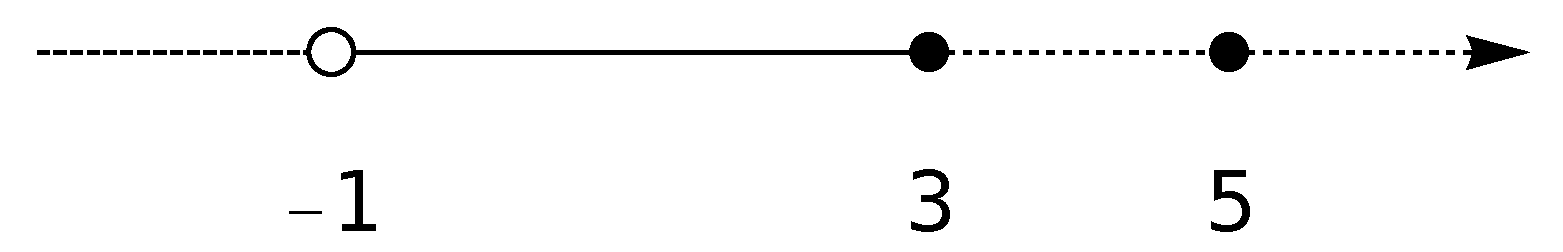
\includegraphics[width=0.4\textwidth]{fig_sets_10c}
		\end{center}
		
	\end{enumerate}
	
	
\end{example}
\fi

\ifcourse
\ifanalysis

	Having introduced the set of real numbers and intervals in $\mathbb{R}$, we are now ready to give a name to some special points in this set, which will turn out useful in the subsequent chapters. 
	\ifcourse
	\checkoddpage
\marginpar{\ifoddpage\hspace*{-1.5cm}\else\hspace*{0.25cm}\fi
\includegraphics[width=0.075\textwidth]{youtube}\\
\ifoddpage\hspace*{-1.75cm}\else\hspace*{0.1cm}\fi
%\includegraphics[width=0.1\textwidth]{Soorten_Punten}
\qrcode[height=1.75cm]{https://youtu.be/U1XDWeeDBrQ}
}
 \fi
	\begin{definition}[Boundary and interior points, open, closed and bounded sets]\label{def:open1D}
		Let $S$ be a set of points in $\mathbb{R}$. A point $P$ in $\mathbb{R}$ is a \textbf{boundary point} (\textit{randpunt}) of $S$  if all open disks centred at $P$ contain both points in $S$ and points not in $S$.\\
		
		A point $P$ in $S$ is an \textbf{interior point} (\textit{inwendig punt}) of $S$ if there is an open interval centred at $P$ that contains only points in $S$. \\
		
		A point $P$ in $S$ is an \textbf{accumulation or limit point} (\textit{ophopingspunt}) of $S$ if the intersection between every open interval containing $P$ and $S$ contain infinitely many points. \\
		
		A set $S$ is \textbf{open} (\textit{open}) if every point in $S$ is an interior point.\\
		
		A set $S$ is \textbf{closed} (\textit{gesloten}) if it contains all of its boundary points.\\
		
		A set $S$ is \textbf{bounded} (\textit{begrensd}) if there is an $M>0$ such that the open interval, centred at the origin with width $M$, contains $S$. A set that is not bounded is unbounded.
		\index{open}\index{closed}\index{open disk}\index{closed disk}\index{boundary point}\index{interior point}\index{bounded set}\index{unbounded set}\index{limit point}\index{accumulation point}
		\index[aut]{inwendig punt}\index[aut]{open bol}\index[aut]{gesloten bol}\index[aut]{open}\index[aut]{gesloten}\index[aut]{begrensd}\index[aut]{onbegrensd}\index[aut]{randpunt}\index[aut]{ophopingspunt}
	\end{definition}

\fi
\fi

\section{Complex numbers}
\label{sec_complex}
We leave a detailed discussion of complex numbers to the course `Algebra', and restrict here to a basic introduction to complex which suffices for the scope of this course. 
	\checkoddpage
\marginpar{\ifoddpage\hspace*{-1.5cm}\else\hspace*{0.25cm}\fi
\includegraphics[width=0.075\textwidth]{youtube}\\
\ifoddpage\hspace*{-1.75cm}\else\hspace*{0.1cm}\fi
\qrcode[height=1.75cm]{https://youtu.be/ysVcAYo7UPI}
}

\subsection{Definition}
Consider the polynomial $p(x) = x^2+1$.  The zeros of $p$ are the solutions to $x^2+1=0$, or $x^2=-1$.  This equation has no real solutions, but we can formally extract the square roots of both sides to get  $x = \pm \sqrt{-1}$.  The quantity $\sqrt{-1}$ is usually relabeled $i$, the so-called \index{imaginary unit} \textbf{imaginary unit} (\textit{imaginaire eenheid}). \index[aut]{imaginaire eenheid}  The number $i$, while not a real number, plays along well with real numbers, and acts very much like any other radical expression.  For instance, $3(2i) = 6i$, $7i-3i = 4i$, $(2-7i) + (3 + 4i) = 5-3i$, and so forth.  The key property that distinguishes $i$ from the real numbers is the fact that  
$$i^2 = -1\,.$$

Hence, if $c$ is a real number with $c \geq 0$, then we can write 
$$\sqrt{-c} = i \sqrt{c}\,.$$

Having defined the imaginary unit, we are now in the position to define the complex numbers.


\begin{definition}[Complex number] \label{complexdefn}
	A \textbf{complex number} (\textit{complex getal}) is a number of the form 
	$$a+bi\,,$$
	where $a$ and $b$ are real numbers and $i$ is the \textbf{imaginary unit} (\textit{imaginaire eenheid}).
\end{definition}
\index{complex number}\index[aut]{complex getal}
\index{imaginary unit}\index[aut]{imaginaire eenheid}

Do not forget that $a$ or $b$ could be zero, which means numbers like $3i$ and $6$ are also complex numbers.  In other words, do not forget that the complex numbers include the real numbers, so $0$ and $\pi - \sqrt{21}$ are both considered complex numbers (See Figure 2.5). 

\subsection{Complex number arithmetic}
The arithmetic of complex numbers is as you would expect, as long as you remember that $i^2=-1$.

\begin{example} 
	\label{complexzeroex1} Perform the indicated operations.  Write your answer in the form $a+bi$.
	\begin{multicols}{2}
		
		
		\begin{enumerate}
			
			\item  $(1-2i) - (3+4i)$
			\item  $(1-2i)(3+4i)$ 
			\item  $\dfrac{1-2i}{3-4i}$
			\item  $\left(x-(1+2i)\right)\left(x-(1-2i)\right)$
			
		\end{enumerate}
	\end{multicols}
	
	\xhrulefill{gray}{2.5pt}Solution \xhrulefill{gray}{2.5pt}
	
	\begin{enumerate}
		
		\item We combine like terms to get $(1-2i) - (3+4i) = 1-2i-3-4i = -2-6i$.
		
		
		\item  Using the distributive property, we get  
		$$
		(1-2i)(3+4i) =3+4i-6i-8i^2\,.
		$$
		
		Since $i^2=-1$, we get $3+4i-6i-8i^2 =  11-2i$.
		
		\item  First we deal with the denominator $3-4i$ as we would any other denominator containing a radical, and multiply both numerator and denominator by $3+4i$.  Doing so produces
		
		\[ \dfrac{1-2i}{3-4i} \;  \dfrac{3+4i}{3+4i} = \dfrac{(1-2i)(3+4i)}{(3-4i)(3+4i)} = \dfrac{11-2i}{25} = \dfrac{11}{25} - \dfrac{2}{25} \, i.\]
		
		
		\item  We can rely on the fact that $(a-b)(a+b)=a^2-b^2$ and see that 
		
		\[\begin{array}{rclr} \left(x-(1+2i)\right)\left(x-(1-2i)\right) & = &  \left((x-1)-2i\right)\left((x-1)+2i\right) & \\
		
		&	= & \left((x-1)^2-(2i)^2\right) & \\ 
		& =  & x^2 -2x +5. & \end{array}\]
		
	\end{enumerate}
	
	
\end{example}

A couple of remarks about the last example are in order.  First, the \index{complex conjugate}\index[aut]{complex toegevoegde}\textbf{conjugate} (\textit{(complex) toegevoegde}) of a complex number $a+bi$ is the number $a-bi$.  The notation commonly used for conjugation is a bar; that is
$$\overline{a+bi} = a-bi\,.$$
For example, $\overline{3+2i} = 3-2i$ and $\overline{6} = 6$.  The properties of the conjugate are summarized below, for $z$ and $w$ complex numbers. 

\begin{itemize}
	
	\item  $\overline{\overline{z}} = z$
	
	\item  $ \overline{z} + \overline{w}  = \overline{z+w}$
	
	\item  $ \overline{z} \, \overline{w}  = \overline{zw}$
	
	\item  $\left(\overline{z}\right)^n = \overline{z^{n}}$, for any natural number $n$
	
	\item  $z$ is a real number if and only if $\overline{z} = z$.
	
\end{itemize}


To form the \textbf{opposite} (\textit{tegengestelde}) of a complex number, take the opposite of each part: 
\[-(a + bi) = -a + (-b)i = -a - bi.\]
For example, the opposite of $6 - 2i$ is $-6 + 2i$. \\


%https://courses.lumenlearning.com/waymakerintermediatealgebra/chapter/read-quadratic-equations-with-complex-solutions/


\ifcourse
Although we will only rarely have to resort to complex numbers throughout this course, their importance in engineering cannot be underestimated since complex numbers have essential  applications in a variety of scientific and related areas such as signal processing, control theory, electromagnetism, fluid dynamics, quantum mechanics, cartography, and vibration analysis. For that reason, you will often encounter them in more advanced mathematics courses, such as differential equations. Besides, using complex numbers one can construct arty and intriguing graphics, like the so-called Julia set depicted in Figure~\ref{fig_sets_11}.
\fi

\ifcourse
\begin{remark}[Quaternions]
	The quaternions are a number system that extends the complex numbers, dating back to the 1840s only. They are generally represented as:
	$$
	a+b\ \mathbf {i} +c\ \mathbf {j} +d\ \mathbf {k}, 
	$$
	where $a$, $b$, $c$, and d are real numbers, and $\mathbf{i}$, $\mathbf{j}$, and $\mathbf{k}$ are the fundamental quaternion units for which it holds that $\mathbf{i}^2=\mathbf{j}^2=\mathbf{k}^2=-1$. Amongst other things, the spin of an electron can be described using quaternions. 	
\end{remark}
\fi

\ifcourse
\begin{figure}[h!]
	\begin{center}
		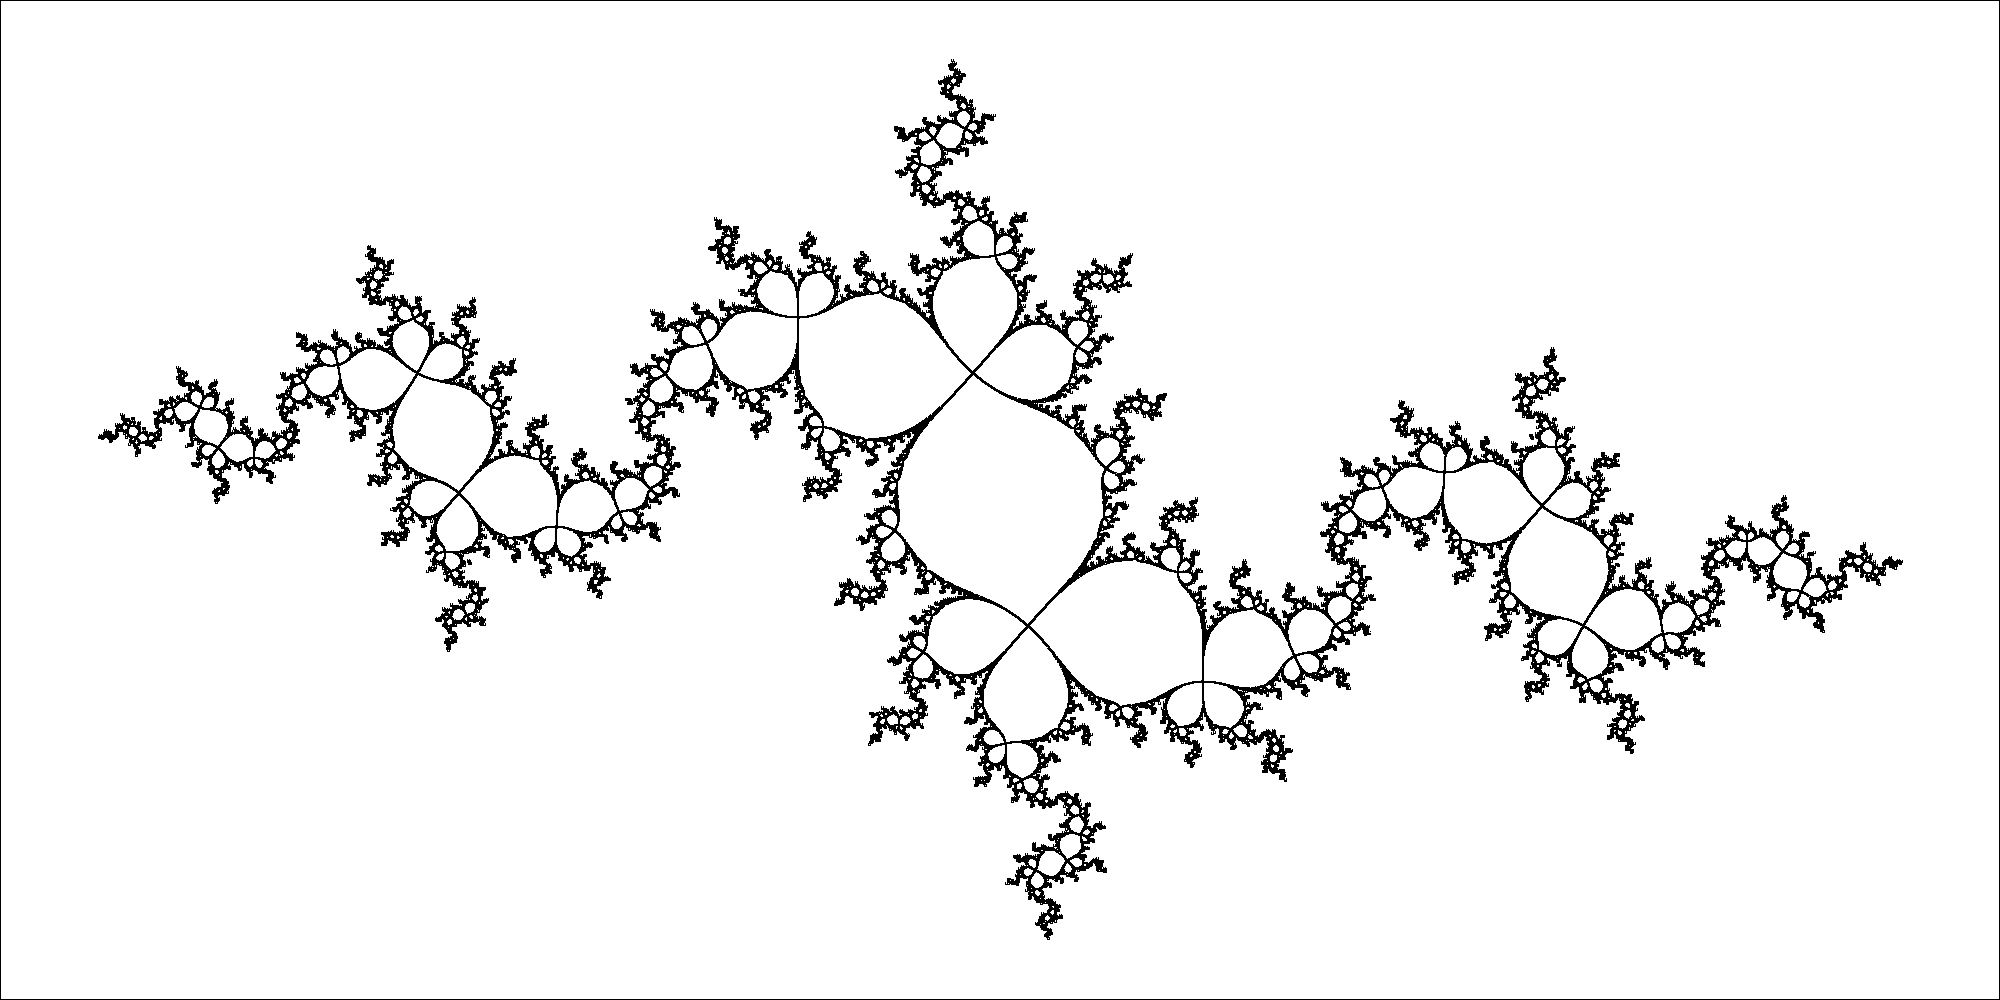
\includegraphics[width=0.7\textwidth]{fig_sets_11}
		\caption{Exemplary Julia set.}
		\label{fig_sets_11}
	\end{center}
\end{figure}
\fi



%Operations and properties of sets, some like the second example and also some with intervals
%A few exercises on sums: http://www.austincc.edu/jthom/SigmaNotationExer.pdf
%Some exercises on powers, roots and special products.
%A few calculations with infinity


%Exercises on exponential growth: http://www.hhofstede.nl/modules/opgavengroei.htm
%http://www.hhofstede.nl/modules/exponentieel%20algemeen.htm

%%%%%%%%%%%%%%%%%%%%%%%%%%
%Exercises in the course
%%%%%%%%%%%%%%%%%%%%%%%%%%

\newpage
\ifcourse %Start of exercises in the course


\section{Exercises}

\renewcommand{\ExerciseListName}{Assignment}

 \subsection*{\nameref{sets} and \nameref{sec:logic operators}}


\ifanalysis\begin{Exercise}[difficulty = 1]\fi
\ifcalculus\begin{Exercise}[difficulty = 2]\fi
Determine the negation of the expressions below.\par 

\begin{multicols}{2}
		\Question $\exists\;x \in \mathbb{Z},\;\forall\;y\in \mathbb{Z}:\;x<y$
		\Question $\forall\;y \in \mathbb{Z},\;\exists\;x\in \mathbb{Z}:\;x<y$
		\Question $\forall\;x \in \mathbb{Z},\;\exists\;y\in \mathbb{Z}:\;x+y=0$
		\Question $\exists\;y \in \mathbb{Z},\;\forall\;x\in \mathbb{Z}:\;x+y=0$
		\EndCurrentQuestion
	\end{multicols}
\ifanalysis\end{Exercise}\fi
\ifcalculus\end{Exercise}\fi
\setboolean{firstanswerofthechapter}{true}
\begin{Answer} \phantom{}
    \begin{multicols}{2}

    	\Question  $\forall \; x \in \mathbb{Z}, \; \exists \; y \in \mathbb{Z}: \; x \geq y $
    	\Question  $\exists\;y \in \mathbb{Z},\;\forall\;x\in \mathbb{Z}:\; x \geq y$
    	\Question  $\exists\;x \in \mathbb{Z},\;\forall\;y\in \mathbb{Z}:\;x+y \neq 0$
    	\Question  $\forall \; y \in \mathbb{Z}, \; \exists\; x \in \mathbb{Z}: \; x+y \neq 0$	
        \EndCurrentQuestion
	\end{multicols}
\end{Answer}
\setboolean{firstanswerofthechapter}{false}

\begin{Exercise}  [difficulty = 1] Define the following sets with words and write them out completely.  
	\begin{multicols}{2}
			\Question $A=\{a\;|\;a\in \mathbb{N} \; \wedge \; 2<a<6 \}$
			\Question $B=\{x\;|\;x\in \mathbb{Q}^+ \; \wedge \; 2x^2 +x-6=0 \}$
			\Question $C=\{x\;|\;x\in \mathbb{Z}^+ \; \wedge \; x^2 -5=0 \}$
			\EndCurrentQuestion
	\end{multicols}
\end{Exercise}

\begin{Answer} \phantom{}
	
    	\Question The set $A$ contains the natural numbers  between 2 and 6. $A = \{3,4,5\}$
    	\Question The set $B$ contains the positive fractions that are solutions of $2x^2 +x-6=0 $. $B = \left\{ \dfrac{3}{2} \right\}$
    	\Question The set $C$ contains the positive integers that are solutions of $x^2-5=0$. $C = \emptyset$
\end{Answer}


\begin{Exercise} Write in a concise manner that $A$ is a set of; 
	\Question[difficulty = 1] all even numbers bigger than 100.
	\Question[difficulty = 1] all pairs of integers whose first and second elements are even and odd, respectively.
	\Question[difficulty = 1] all integers, different from zero, that are multiples of 3.
	\Question[difficulty = 1] all positive rational numbers whose square root is greater than 3.
	\Question[difficulty = 2] all numbers that when divided by 6 result in a remainder of 2.
\end{Exercise}

\begin{Answer}\phantom{}
    \begin{multicols}{2}

    		\Question $A = \left\{a\; \left|\; \dfrac{a}{2}\in \mathbb{N} \; \wedge \; a > 100 \right. \right\}$
    		\Question $A = \left\{(a,b)\; \left|\; a,b \in \mathbb{Z} \; \wedge \; \dfrac{a}{2} \in \mathbb{Z} \; \wedge \; \dfrac{b+1}{2} \in \mathbb{Z} \right. \right\}$
            \Question $A = \left\{a\; \left|\; a\in \mathbb{Z}_0 \; \wedge \; \dfrac{a}{3}\in \mathbb{Z}_0 \right. \right\}$  %all even numbers, different from zero, that are multiples of 3.
            \Question $A = \left\{a\; \left|\; a\in \mathbb{Q}^+ \; \wedge \; \sqrt{a}>3 \right. \right\}$ 
            \Question $A = \left\{a\; \left|\; a\in \mathbb{R} \; \wedge \; \dfrac{a-2}{6} \in \mathbb{Z} \right. \right\}$
    	\EndCurrentQuestion
    \end{multicols}
\end{Answer}
	
\begin{Exercise} Fill in the correct symbols. Choose from $\subset, \not\subset, =, \neq, \in,  \not\in, \ni, \not\ni$. Multiple answers might be possible.
	\Question[difficulty = 1] $\{1, 3, 5, 7, 9, 11, \ldots \} \ldots \{ x \in \mathbb{N} | \; x \text{ is an even number} \}$
	\Question[difficulty = 1] $\{ x | \; x \text{ is a rose} \} \ldots \{ x | \; x \text{ is a flower} \}$
	\Question[difficulty = 1] $\{1, 3, 5, 7, 9 \} \ldots 2$
	\Question[difficulty = 1] $\{1\} \ldots \{1, 3, 5, 7, 9 \} $
	\Question[difficulty = 1] $\{1,3\} \ldots \{\{1\}, \{3\}, \{5\}, \{7\}, \{9\} \} $
	\Question[difficulty = 1] $\{1,3\} \ldots \{1, 3, 5, 7, 9 \} $
	\Question[difficulty = 1] $\{1, 3, 5, 7, 9 \} \ldots \emptyset$
	\ifanalysis\Question[difficulty = 1]\fi \ifcalculus\Question[difficulty = 2]\fi $\{1\} \ldots \{\{1\}, \{3\}, \{5\}, \{7\}, \{9\} \} $
	\Question[difficulty = 2] $\{1, 3, \{5, 7, 9\} \} \ldots 5$
\end{Exercise}

\begin{Answer}\phantom{}

    		\Question $\{1, 3, 5, 7, 9, 11, \ldots \} = \{ x \in \mathbb{N} | \; x \text{ is an odd number} \}$
    		\Question $\{ x | \; x \text{ is a rose} \} \subset \{ x | \; x \text{ is a flower} \}$
    		\Question $\{1, 3, 5, 7, 9 \} \not\ni 2$
    		\Question $\{1\} \subset \{1, 3, 5, 7, 9 \} $
    		\Question $\{1,3\} \not\subset \{\{1\}, \{3\}, \{5\}, \{7\}, \{9\} \} $ also $\{1,3\} \not\in \{\{1\}, \{3\}, \{5\}, \{7\}, \{9\} \} $
    		\Question $\{1,3\} \subset \{1, 3, 5, 7, 9 \} $
    		\Question $\{1, 3, 5, 7, 9 \} \neq \emptyset$
    		\Question $\{1\} \in \{\{1\}, \{3\}, \{5\}, \{7\}, \{9\} \} $
    		\Question $\{1, 3, \{5, 7, 9\} \} \not\ni 5$

\end{Answer}

\newpage

\begin{Exercise} Assume $A=\{1, \{1\}, \{2\} \}$. Which from the following statements is true?
    \begin{multicols}{2}
    	\Question[difficulty = 1] $1 \in A$
    	\ifanalysis\Question[difficulty = 1]\fi \ifcalculus\Question[difficulty = 2]\fi $\{1\} \in A$
    	\ifanalysis\Question[difficulty = 1]\fi \ifcalculus\Question[difficulty = 2]\fi $\{1\} \subseteq A$
    	\ifanalysis\Question[difficulty = 1]\fi \ifcalculus\Question[difficulty = 2]\fi $\{\{1\}\} \subseteq A$
    	\ifanalysis\Question[difficulty = 1]\fi \ifcalculus\Question[difficulty = 2]\fi $2 \in A$
    	\ifanalysis\Question[difficulty = 1]\fi \ifcalculus\Question[difficulty = 2]\fi $\{\{2\}\} \subseteq A$	
    	\ifanalysis\Question[difficulty = 1]\fi \ifcalculus\Question[difficulty = 2]\fi $\{\{2\}\} \subset A$
    	\Question[difficulty = 2] $\{2\} \subseteq A$
    	\EndCurrentQuestion
	\end{multicols}
\end{Exercise}

\begin{Answer}\phantom{}
    \begin{multicols}{2}
        
        	\Question $1 \in A$: True
        	\Question $\{1\} \in A$: True
        	\Question $\{1\} \subseteq A$: True
        	\Question $\{\{1\}\} \subseteq A$: True
        	\Question $2  \in A$: False 
        	\Question $\{\{2\}\} \subseteq A$: True	
        	\Question $\{\{2\}\} \subset A$: True	
        	\Question $\{2\} \subseteq A$: False
        \EndCurrentQuestion
    \end{multicols}
\end{Answer}

\begin{Exercise} 
    Given $U=\{1, 2, 3, \ldots, 9, 10\}$, assume $A =\{1, 2, 3, 4, 5\}$, $B =\{1, 2, 3, 4\}$, $C =\{3, 5, 7\}$ and $D =\{2, 4, 6, 8\}$. Describe each of the following sets:
    \begin{multicols}{2}
    	\Question[difficulty = 1] $(A \cup B) \cap C$
    	\Question[difficulty = 1] $A \cup (B \cap C)$
    	\Question[difficulty = 1] $\overline{C} \cup \overline{D}$
    	\Question[difficulty = 1] $\overline{C \cap D}$
    	\Question[difficulty = 1] $(A \cup B)\backslash C $
    	\Question[difficulty = 1] $A \cup (B \backslash C)$
    	\ifanalysis\Question[difficulty = 1]\fi \ifcalculus\Question[difficulty = 2]\fi $(B \backslash C) \backslash D$	
    	\ifanalysis\Question[difficulty = 1]\fi \ifcalculus\Question[difficulty = 2]\fi $B \backslash (C \backslash D)$
    	\Question[difficulty = 2] $(A \cup B)\backslash (C \cap D) $
    	\EndCurrentQuestion
	\end{multicols}
\end{Exercise}

\begin{Answer}\phantom{}
    \begin{multicols}{2}
    
        	\Question $(A \cup B) \cap C = \{3, 5\}$
        	\Question $A \cup (B \cap C) = \{1, 2, 3, 4, 5\} = A$
        	\Question $\overline{C} \cup \overline{D} = U$
        	\Question $\overline{C \cap D} = \overline{C} \cup \overline{D} = U $ \quad (rules of De Morgan)
        	\Question $(A \cup B)\backslash C = \{1, 2, 4\} $
        	\Question $A \cup (B \backslash C) = \{1, 2, 3, 4, 5\} = A$
        	\Question $(B \backslash C) \backslash D = \{1\}$	
        	\Question $B \backslash (C \backslash D) = \{1, 2, 4\}$
            \Question $(A \cup B)\backslash (C \cap D) = \{1, 2, 3, 4, 5\} = A$
        \EndCurrentQuestion
    \end{multicols}
\end{Answer}

\begin{Exercise} Simplify the following expressions:
    \begin{multicols}{2}
    	\Question[difficulty = 1] $A \cap (B \backslash A)$
    	\Question[difficulty = 1] $(A \backslash B) \cup (A \cap B)$
    	\Question[difficulty = 2] $\overline{A} \cup \overline{B} \cup \left( A \cap B \cap \overline{C} \right)$
    	\Question[difficulty = 3] $(A \cap B) \cup \left( A \cap B \cap \overline{C} \cap D \right) \cup \left( \overline{A} \cap B \right)$
    	\Question[difficulty = 3] $(A \cap B) \cup \left(B \cap \left( \left(C\cap D\right)\cup \left(C \cap \overline{D} \right) \right)   \right)$
    	\EndCurrentQuestion
	\end{multicols}
\end{Exercise}

\begin{Answer}\phantom{}
    
        \Question $A \cap (B \backslash A) = \emptyset $
        \Question $(A \backslash B) \cup (A \cap B) = A$
        \Question $\overline{A} \cup \overline{B} \cup \left( A \cap B \cap \overline{C} \right) = \overline{A \cap B \cap C}$
        \Question $(A \cap B) \cup \left( A \cap B \cap \overline{C} \cap D \right) \cup \left( \overline{A} \cap B \right) = B$
        \Question $(A \cap B) \cup \left(B \cap \left( \left(C\cap D\right)\cup \left(C \cap \overline{D} \right) \right) \right) = (A \cap B) \cup (B \cap C) $
\end{Answer}

%%%%%%%%%%%%%%
%Only bio-ir
\ifanalysis


\begin{Exercise} [difficulty = 1] Prove the associative properties with respect to union and intersection for three sets. 
\end{Exercise}

\begin{Answer}\phantom{}
The answer is left as an exercise to the reader. 
\end{Answer}
		
\begin{Exercise} Prove the following properties. %
		\Question[difficulty = 1] $A\cup B=B \; \Leftrightarrow \; A\subset B \; \Leftrightarrow\;  A\cap
		B=A \; \Leftrightarrow \; A\backslash B=\emptyset$
		\Question[difficulty = 1] $A\backslash B=A \; \Leftrightarrow \; A \cap B =\emptyset \; \Leftrightarrow \;
		B \backslash A=B$
		\Question[difficulty = 1] $(A\backslash B)\cap A=A\backslash B$
		\Question[difficulty = 1] $(A\backslash B)\cap B=\emptyset$
		\Question[difficulty = 1] $(A\cup B)\backslash B=A\backslash B$
		\Question[difficulty = 1] $(A\cup B)\backslash C=(A\backslash C)\cup (B\backslash C)$
		%\Question $(A\cap B)\backslash C=(A\backslash C)\cap (B\backslash C)$
\end{Exercise}

\begin{Answer}\phantom{}
The answer is left as an exercise to the reader.
\end{Answer}


\fi
%%%%%%%%%%%%%%
\newpage

\begin{Exercise} [difficulty = 2, label=oef_fig_sets_12] Use set notation to define the shaded areas in Figure~\ref{fig_sets_12}. \label{oef_verz} 
	\begin{figure}[H]
		\begin{center}
			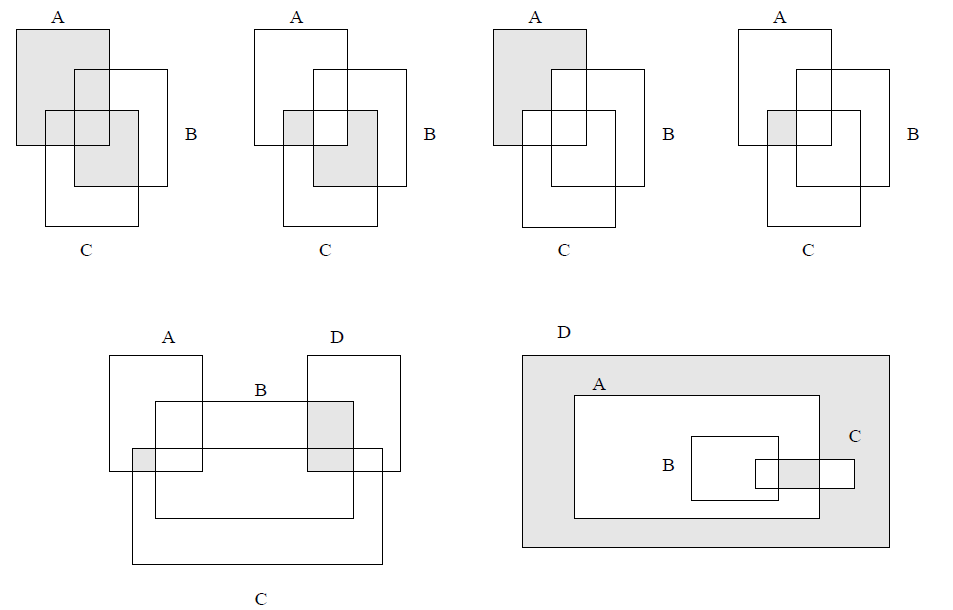
\includegraphics[width=0.9\textwidth]{fig_sets_12}
			\caption{Shaded areas used in exercise~\ref{oef_fig_sets_12}.}
			\label{fig_sets_12}
		\end{center}
	\end{figure}
\end{Exercise}

\begin{Answer}\phantom{}
    The numbering of the areas is done from left to right.
    	\begin{multicols}{2}
    
        	\Question $A \cup (B \cap C) $
        	\Question $((B \cap C) \backslash A) \cup  ((A \cap C) \backslash B) $
        	\Question $ A \backslash (B \cup C)$ of $ (A \backslash B) \cap (A \backslash C)$
        	\Question $(A \cap C) \backslash B$
        	\Question $((A \cap C) \backslash B) \cup (B \cap D) $
        	\Question $(D \backslash (A \cup C)) \cup ((C \cap A) \backslash B) $
        	\EndCurrentQuestion
    	\end{multicols}
\end{Answer}

%%%%%%%%%%%%%%
%Only bio-ir.
\ifanalysis

\begin{Exercise} Assume $W \subset \mathbb{R}$ and $b \in \mathbb{R}$. Give a correct expression with logical operators for the expressions below. 
		\Question[difficulty = 1] $b$ is an upper limit of set $W$.
		\Question[difficulty = 1] $b$ is not an upper limit of set $W$.
		\Question[difficulty = 2] $W$ is an upwardly bounded set.
		\Question[difficulty = 2] $W$ is not an upwardly bounded set.
\end{Exercise}

\begin{Answer}\phantom{}

    \Question $b$ is an upper bound of the set $W$: \quad $\forall w \in W: w \leq b$
    \Question $b$ is not an upper bound of the set $W$: \quad $\exists w \in W: b < w$
    \Question $W$  is a set bounded from above: \quad $\exists b \in \mathbb{R} | \forall w \in W: w \leq b$
    \Question $W$ is a set not bounded from above: \quad $\forall b \in \mathbb{R} : \exists w \in W: b < w$
\end{Answer}
		
\begin{Exercise} \\Determine the supremum and infimum of the following subsets of $\mathbb{R}$. 
    \begin{multicols}{3}
		%Ex. 1.10 pg 52 course calculus and analysis JB
		\Question[difficulty = 1] $\left\{ \dfrac{2^n}{2^n+1}, \, n \in \mathbb{N}  \right\}$
		\Question[difficulty = 1] $\left\{ \dfrac{2n-1}{n+2}, \, n \in \mathbb{N}_0  \right\}$
		\Question[difficulty = 1] $\left\{ \dfrac{n}{n+1}, \, n \in \mathbb{N}  \right\}$
		\EndCurrentQuestion
	\end{multicols}
\end{Exercise}

\begin{Answer}\phantom{}
    \begin{multicols}{2}

    \Question inf = $1/2$, sup = $1$
    \Question inf = $1/3$, sup = $2$
    \Question inf = $0$, sup = $1$
    \EndCurrentQuestion
    \end{multicols}
\end{Answer}
		
\subsection*{\nameref{intervals}}		
		
\begin{Exercise} Determine the infimum, supremum, minimum, maximum, boundary points, and interior points of $A$. 
    \begin{multicols}{2}
		\Question[difficulty = 1] $A = \{1\} \cup [2,5[ \; \cup \; ]5,7[$
		\Question[difficulty = 1] $A = \{-3\}\, \cup\; ]0,4] \; \cup \; [7,+\infty[$
		\Question[difficulty = 1] $A =\; ]-\infty,-2[ \; \cup \; ]-2,2[ \; \cup \; [3,4[ \; \cup \; ]5,9]$
		\EndCurrentQuestion
	\end{multicols}
\end{Exercise}

\begin{Answer}\phantom{}

    \Question inf $A=1$, sup $A=7$, min $A=1$, max $A$ does not exist, boundary points $A: 1, 2, 5, 7$, \\ internal points $A:\; ]2,5[ \;\cup\; ]5,7[$
    \Question inf $A=-3$, sup $A$ does not exist, min $A=-3$, max $A$ does not exist, \\ boundary points $A: -3, 0, 4, 7$, internal points $A: \; ]0,4[ \; \cup \; ]7,+\infty[$
    \Question inf $A$ does not exist, sup $A=9$, min $A$ does not exist, max $A=9$, \\ boundary points $A: -2, 2, 3, 4, 5, 9$, \\ internal points $A:\; ]-\infty,-2[\; \cup\; ]-2,2[\;\cup\; ]3,4[ \;\cup\; ]5,9[$
\end{Answer}
		
\fi
%%%%%%%%%%%%%%

\subsection*{\nameref{sec_real}}

\begin{Exercise}[difficulty = 1] Which of the numbers below are rational or irrational?
	\begin{multicols}{2}
			\Question $5.369$
			\Question $\dfrac{12}{7}$
			\Question $\sqrt{13}$
			\Question $1.232345456767\ldots$
			\Question $3.0236363636\ldots$
			%	\Question $\dfrac{\pi}{3}$
			%	\Question $-6.147258369\ldots$
			\Question $\sqrt{121}$
		    \EndCurrentQuestion
	\end{multicols}
\end{Exercise}

\begin{Answer}\phantom{}
    \begin{multicols}{3}
		
			\Question rational
			\Question rational
			\Question irrational
			\Question irrational
			\Question rational
			\Question rational
		\EndCurrentQuestion 
	\end{multicols}
\end{Answer}
	
\begin{Exercise} Rewrite the following expressions using a sum or multiplication sign.
    \begin{multicols}{2}
    	\Question[difficulty = 1] $x + x^2 + x^3 + x^4 + \ldots + x^{99}$ 
    	\Question[difficulty = 1] $\sqrt{3} + \sqrt{5} + \sqrt{7} + \sqrt{9} + \ldots + \sqrt{51} $ 
    	\Question[difficulty = 1] $ \dfrac{1}{a+1} \cdot \dfrac{4}{a+2} \cdot \dfrac{9}{a+3} \cdot \dfrac{16}{a+4}  \cdots  \dfrac{169}{a+13}$
    	\EndCurrentQuestion
    \end{multicols}
\end{Exercise}

\begin{Answer}\phantom{}
    \begin{multicols}{3}
		
		\Question $\dsum_{j=1}^{99} x^j$ 
		\Question $\dsum_{j=1}^{25} \sqrt{2j+1}$ 
		\Question $\displaystyle\prod_{j=1}^{13} \dfrac{j^2}{a+j}$ 
	    \EndCurrentQuestion
	\end{multicols}
\end{Answer}
	
\begin{Exercise} Calculate the following sums.
    \begin{multicols}{3}
    	\Question[difficulty = 1] $\dsum_{j=0}^{3} 2^j$
    	\Question[difficulty = 1] $\dsum_{j=0}^{3} j^2$
    	%\item $\dsum_{j=1}^{5} (2j-3)$
    	\Question[difficulty = 1] $\dsum_{j=0}^{4} \dfrac{24}{j!}$
    	\Question[difficulty = 1] $\dsum_{j=1}^{4} \dfrac{(-1)^j}{j}$
    	\Question[difficulty = 1] $\dsum_{j=1}^{5} (2j-1)^2$
    	\ifanalysis\Question[difficulty = 1]i\fi \ifcalculus\Question[difficulty = 2]\fi $\dsum_{j=1}^{100} -7j^2$
    	\ifanalysis\Question[difficulty = 1]\fi \ifcalculus\Question[difficulty = 2]\fi $\dsum_{j=1}^{90} \left(-2j^2+3j-5\right)$
    	\ifanalysis\Question[difficulty = 1]\fi \ifcalculus\Question[difficulty = 2]\fi $\dsum_{\stackrel{0<k<10}{k \text{ is oneven}}} k^2$
    	\EndCurrentQuestion
	\end{multicols}
\end{Exercise}

\begin{Answer}\phantom{}
    \begin{multicols}{3}
		
			\Question $15$ 
			\Question $14$ 
			\Question $65$ 
			\Question $- \dfrac{7}{12}$ 
			\Question $165$ 
			\Question $-2368450$
			\Question $-482295$  
		    \Question $165$ 
		\EndCurrentQuestion
	\end{multicols}
\end{Answer}
	
\begin{Exercise} Simplify each sum or product to an expression without sigma or pi notation. 
    \begin{multicols}{2}
    	\Question[difficulty = 1] $\dsum_{j=1}^{n} (3j-2)$
    	\Question[difficulty = 1] $\dsum_{j=1}^{n} \left( (3j-5)\,\dfrac{1}{n^2} \right)$		
    	\ifanalysis\Question[difficulty = 1]\fi \ifcalculus\Question[difficulty = 2]\fi $\dsum_{j=1}^{n} (3j-4)^2$
    	\ifanalysis\Question[difficulty = 1]\fi \ifcalculus\Question[difficulty = 2]\fi $\dsum_{j=1}^{n} \left( (j-2)^2\,\dfrac{1}{n^3} \right)$
    	\Question[difficulty = 2] $\displaystyle\prod_{j=1}^{n} j^3$
    	\Question[difficulty = 3] $\displaystyle\prod_{k=2}^{n} \left(1- \dfrac{1}{k^2} \right)$
    	\EndCurrentQuestion
    \end{multicols}
\end{Exercise}

\begin{Answer}\phantom{}
    \begin{multicols}{2}
		
			\Question $\dfrac{n(3n-1)}{2}$
			\Question $\dfrac{3n-7}{2n}$
			\Question $\dfrac{n}{2}(6n^2-15n+11)$	
			\Question $\dfrac{(n+1)(2n-11)+24}{6n^2}$
            \Question $\left(n!\right)^3$ 
		    \Question $\dfrac{n+1}{2n}$ 
		\EndCurrentQuestion
	\end{multicols}
\end{Answer}

\ifanalysis\pagebreak\fi

\begin{Exercise} Calculate or simplify the following algebraic forms.
    \begin{multicols}{2}
    	\Question[difficulty = 1] $\left(64\;a^{6m}b^{12n}c^{18p}\right)^{\frac{1}{6}}$
    	\Question[difficulty = 1] $\dfrac{1-x}{1-\sqrt{x}}$
    	\Question[difficulty = 1] $\left(1-\sqrt{2}-\sqrt{3}\right)^2$
    	\Question[difficulty = 1] $b\sqrt{\dfrac{4a}{b^4}}-\sqrt{\dfrac{9a}{b^2}}+\dfrac{1}{b}\sqrt{\dfrac{a}{4}}+2b\sqrt{\dfrac{25a}{b^4}}$
    	\ifanalysis\Question[difficulty = 1]\fi \ifcalculus\Question[difficulty = 2]\fi $\left(\sqrt{\dfrac{x+1}{x-1}}\right) \left( \sqrt[3]{\dfrac{x-1}{x+1}}\right)$
    	\ifanalysis\Question[difficulty = 1]\fi \ifcalculus\Question[difficulty = 2]\fi $\sqrt[3]{a^3+\dfrac{3}{2}a^2b+\dfrac{3}{4}ab^2+\dfrac{1}{8}b^3}$
    	\ifanalysis\Question[difficulty = 1]\fi \ifcalculus\Question[difficulty = 2]\fi $\dfrac{a^2+b^2}{\left(b-a\right)^2}\,\dfrac{\left(a-b\right)^3}{a+b}\,\dfrac{\left(-a-b\right)^2}{a^2-b^2}$
    	\ifanalysis\Question[difficulty = 1]\fi \ifcalculus\Question[difficulty = 2]\fi $\left(x^{\frac{1}{3}}-x^{-\frac{1}{3}}\right)^3+3\left(x^{\frac{1}{3}}-x^{-\frac{1}{3}}\right)$
    
    	\ifanalysis\Question[difficulty = 1]\fi \ifcalculus\Question[difficulty = 2]\fi $ \dfrac{\left(x^2 \right)^3 x^{-4} \sqrt[3]{x^5}}{\sqrt[3]{x^2} \sqrt[3]{\sqrt[4]{\left(x^2 \right)^3}}} $
    	\Question[difficulty = 2] $\left( \dfrac{16^{-2} a^{\frac{1}{2}}b^{-3}}{81^{-1} a^{-\frac{1}{2}}b^{3}} \right) \sqrt{ab^{\frac{9}{4}} \left( ab^{\frac{3}{2}} \right)^{\frac{1}{2}}}  $
    	\EndCurrentQuestion
	\end{multicols}
\end{Exercise}

\begin{Answer}\phantom{}
    \begin{multicols}{2}
	
		\Question $2 a^m b^{2n} c^{3p}$
		\Question $1+\sqrt{x}$
		\Question $6-2\sqrt{2}-2\sqrt{3}+2\sqrt{2}\sqrt{3}$
		\Question $\dfrac{19\sqrt{a}}{2b}$
		\Question $ \sqrt[6]{\dfrac{x+1}{x-1}}$
		\Question $a + \dfrac{b}{2}$
		\Question $a^2+b^2$
		\Question $\dfrac{x^2-1}{x}$
		\Question $x^{\frac{5}{2}} $ 
		\Question $\dfrac{81}{256} a^{\frac{7}{4}} b^{-\frac{9}{2}}$ 
	\EndCurrentQuestion
	\end{multicols}
\end{Answer}

\subsection*{\nameref{sec_complex}}

\begin{Exercise}[difficulty = 1] Determine and simplify
	\begin{multicols}{3}	
		\begin{itemize}[labelsep=5mm]	
			\item  $z+w$
			\item  $zw$
			\item  $z^2$	
			\item  $z^{-1}$
			\item  $\dfrac{z}{w}$
			\item  $\dfrac{w}{z}$
			\item  $\bar{z}$
			\item  $z\bar{z}$
			\item  $\left(\bar{z}\right)^2$
		\end{itemize}
	\end{multicols}
rewrite each pair of complex numbers in standard  form: $a+bi$.  
	\begin{multicols}{2}
			\Question  $z = 2+3i$, \quad $w = 4i$
			\Question  $z = 1+i$, \quad $w = -i$
			\Question  $z = 3-5i$, \quad $w = 2+7i$
			\Question  $z = \sqrt{2}-\sqrt{2}i$, \quad $w = \sqrt{2}+\sqrt{2}i$
			\Question  $z = 1-\sqrt{3}i$, \quad $w = -1-\sqrt{3}i$
			\Question  $z = -\dfrac{\sqrt{2}}{2} + \dfrac{\sqrt{2}}{2} i$, \quad $w =  -\dfrac{\sqrt{2}}{2} - \dfrac{\sqrt{2}}{2} i$
		\EndCurrentQuestion
	\end{multicols}
\end{Exercise}

\begin{Answer}\phantom{} \newline
    \vspace{-0.6cm} \begin{small} $\renewcommand{\arraystretch}{1.15}\begin{array}{|c|c|c|c|c|c|c|c|c|c|}			\hline
			&&&&&&\vspace{-0.5cm}\\
			& z+w & zw & z^2 & z^{-1} &\dfrac{z}{w} & \dfrac{w}{z} & \bar{z} & z\bar{z} & \left(\bar{z}\right)^2 \\
			&&&&&&\vspace{-0.5cm}\\
			\hline
			\hline
			&&&&&&\vspace{-0.5cm}\\
			\mbox{(a)}  & 2+7i & 8i  & -5+12i&  \dfrac{2-3i}{13} & \dfrac{3-2i}{4} & \dfrac{12+8i}{13}  & 2-3i & 13 & -5-12i \\[0.3cm]
			\hline 
			\mbox{(b)} & 1 & 1-i & 2i & \dfrac{1-i}{2}& -1+i & \dfrac{-1-i}{2} & 1-i & 2 &-2i \\[0.3cm]
			\hline
			\mbox{(c)} & 5+2i & 41+11i & -16-30i & \dfrac{3+5i}{34} & \dfrac{-29-31i}{53} & \dfrac{-29+31i}{34} & 3+5i & 34 & -16+30i \\[0.3cm]
			\hline
			\mbox{(d)} & 2\sqrt{2} & 4 &  -4i  & \dfrac{\sqrt{2}+\sqrt{2}i}{4} & -i & i & \sqrt{2}+\sqrt{2}i & 4 & 4i \\[0.3cm]
			\hline
			\mbox{(e)} & -2\sqrt{3}i & -4 &  -2-2\sqrt{3}i  & \dfrac{1+\sqrt{3}i}{4} & \dfrac{1+\sqrt{3}i}{2} & \dfrac{1-\sqrt{3}i}{2} & 1+\sqrt{3}i & 4 & -2+2\sqrt{3}i \\[0.3cm]
			\hline
			\mbox{(f)} & -\sqrt{2} & 1 &  -i  & \dfrac{-\sqrt{2}-\sqrt{2}i}{2} & -i & i & \dfrac{-\sqrt{2}-\sqrt{2}i}{2} & 1 & i \\[0.3cm]
			\hline
			\end{array}$
		\end{small}
\end{Answer}

%\ifcalculus\newpage\fi

\begin{Exercise} Write the following numbers in standard form: $a+bi$.
    \begin{multicols}{2}
    	\Question[difficulty = 1] $(4+8i)+(15-12i)$
    	\Question[difficulty = 1] $(2+4i)-(6-7i)$
    	\Question[difficulty = 1] $(2+3i)+(-5+i)$
    	\Question[difficulty = 1] $(2+i)^2$
    	\Question[difficulty = 1] $\overline{(5+6i)}(5+6i)$
    	\Question[difficulty = 1] $\dfrac{1}{5+2i}$
    	\Question[difficulty = 1] $\dfrac{1+i}{2+3i}$
    	\ifanalysis\Question[difficulty = 1]\fi \ifcalculus\Question[difficulty = 2]\fi $\dfrac{1+2i}{3-4i} + \dfrac{2-i}{5i}$	
    	\EndCurrentQuestion
	\end{multicols}
\end{Exercise}

\begin{Answer}\phantom{}
    \begin{multicols}{3}
	
		\Question $19-4i$
		\Question $-4+11i$
		\Question $-3+4i$
		\Question $3+4i$
		\Question $61$
		\Question $\dfrac{5-2i}{29}$
		\Question $\dfrac{5-i}{13}$
		\Question $\dfrac{-2}{5}$	
	\EndCurrentQuestion
	\end{multicols}
\end{Answer}

\fi 
%End of the exercises in the course

